\section{Collusion: Forms, Law, and Facts}\label{sec:12-facts}

Firms that sell substitutes can earn more by acting together than by competing. When they succeed, prices rise
above the competitive level and buyers pay the difference. This section fixes the vocabulary and explains how
economists model collusion. It then asks when tacit collusion fails, describes how the law treats collusion, and
summarizes what the records of enforcement agencies show. \Cref{sec:12-repeated} then
develops the theory of repeated games. \Cref{sec:12-perfect} applies it to the simplest environment, in which every
firm observes what its rivals did.

\subsection{Forms of collusion}\label{sec:12-forms}

\begin{definition}[Collusion]\label{def:12-collusion}
\emph{Collusion} is coordination among competing firms that raises prices, restricts output, or divides markets
relative to the non-cooperative outcome of their market game. A \emph{cartel} is an organized group of firms that
colludes.
\end{definition}

The non-cooperative outcome in the definition is the static Nash equilibrium of the game that the firms play in a
single period. It is an equilibrium in prices when firms set prices, in quantities when they set quantities, and in
bids when they compete in an auction. Collusion is always measured against this benchmark. In the homogeneous
Bertrand model of \cref{sec:02-bertrand} the benchmark price is marginal cost, so any price above marginal cost is
collusive.

Collusion takes several forms. \emph{Price fixing} is an agreement on prices, on price increases, or on minimum
prices. \emph{Bid rigging} is collusion in auctions and procurement, where the colluders decide in advance who will
win and at what bid. \emph{Market division} allocates customers, territories, or sales quotas among the firms, so
that each firm faces less competition for its share. The forms are often combined. Most documented cartels agree on
prices and also allocate sales among their members, as \cref{sec:12-cartels} shows.

Economists distinguish two ways of reaching a collusive outcome. \emph{Explicit collusion} uses direct
communication and agreement among the firms, such as meetings to set prices, exchanges of sales data, and payments
between cartel members. \citet[p.~ix]{MarshallMarx2012} define it as an agreement among competitors that relies on
interfirm communication or transfers to suppress rivalry. \emph{Tacit collusion} sustains prices above the static
Nash level as a non-cooperative equilibrium of a repeated game, without any explicit agreement. In the words of
\citet[p.~9]{MarshallMarx2012}, tacit collusive equilibria are those that need no direct interaction between the
firms, such as communication or transfers. The distinction concerns the means of coordination.
The logic of enforcement is the same in both cases: a firm refrains from undercutting because undercutting would
provoke a costly response from its rivals. \Cref{sec:12-perfect} shows that this logic needs no communication at all
when firms observe each other's prices. Communication becomes valuable when firms hold private information about
costs, demand, or their own sales (\cref{sec:12-private-costs,sec:12-cartels}).

Collusion can also occur on the buying side of a market. A \emph{buyer cartel} colludes to depress the prices its
members pay for an input, which is collusion among buyers with monopsony power. A \emph{no-poach agreement} is a
pledge among employers not to hire each other's workers, which is collusion in a labor market. The theory of this
chapter applies to both, with the direction of the price distortion reversed.

\subsection{How economists model collusion}\label{sec:12-modelling}

The modern theory of collusion starts from non-cooperative behavior. It takes the static Nash equilibrium as the
outcome that firms would reach if they met only once. It then takes seriously that the same firms meet again and
again. A firm that cuts its price today gains sales today, but it may provoke a price war that lowers its profit for
many periods. If the future matters enough, the threat of such a war can sustain high margins today, even though
every firm could gain in the short run by cutting its price \citep{Friedman1971}.

The workhorse model is an infinitely repeated game. A fixed set of firms plays the same stage game in every period
and discounts future profits. The model abstracts from entry and exit, from investment, and from the evolution of
demand and technology. Later sections relax some of these simplifications. Demand fluctuates in
\cref{sec:12-demand}, and firms observe their rivals imperfectly in
\cref{sec:12-public,sec:12-private-costs,sec:12-cartels}.

Two consequences of this approach shape the whole chapter. First, collusion is a property of an equilibrium, so it
requires neither a contract nor even a conversation. Second, repeated games have many equilibria. The theory tells
us which outcomes can be sustained, but it does not tell us which outcome firms will reach. This multiplicity is a
central difficulty for empirical work on collusion, to which \cref{ch:collusion-evidence} returns.

Game theory draws a line that is easy to misread in legal debates. \emph{Cooperative games} allow binding
agreements, whose enforcement lies outside the analysis. \emph{Noncooperative games} allow none
\citep[p.~177]{Kaplow2013}. Competition law makes every price-fixing agreement unenforceable in court, so the
oligopoly problem belongs to noncooperative theory. That theory covers express cartels with detailed negotiated
agreements, the pure interdependence of two gas stations that watch each other's signs, and everything in between
(p.~178). Economists also call the outcomes of a noncooperative game cooperative or noncooperative, and the double use
invites confusion. \citet[p.~20]{Friedman1986}, quoted by \citet[p.~179]{Kaplow2013}, keeps the two apart: ``The
presence or absence of binding agreements is the definitive element for cooperative versus noncooperative games.''
A collusive outcome of a repeated game is therefore cooperative in its payoffs and noncooperative in its structure.
When an economist says that a cartel in a repeated game has no agreement, the word means a binding contract. The
legal notion of agreement is broader and covers at least classic cartels (pp.~180--181). \Cref{sec:12-kaplow} asks
whether game theory offers any narrower notion that could separate legal from illegal coordination.

\subsection{When tacit collusion fails}\label{sec:12-tacit-fails}

If repeated interaction can sustain the monopoly price without a conversation, why do firms ever take the legal
risk of explicit collusion? \citet[pp.~9--17]{MarshallMarx2012} answer with a sequence of examples in which they
remove or restore communication and transfers. \Cref{tab:12-mm-scenarios} summarizes them and names the model of this
chapter that formalizes each one.

The first two examples concern two gas stations on opposite corners of a small town. The nearest rival vendor is at least
150 miles away. Each station buys gasoline at \$2 per gallon, and a common price of \$3 maximizes joint profit. Prices are
posted at 6 AM and cannot change until the next morning (p.~10). In a static setting each station undercuts any
common price above cost by one cent, and the only equilibrium price is \$2.01. When the future matters, each station
expects that an undercut will lead its rival to give up on high prices, and both post \$3 (p.~11). The outcome is the
one that private communication could achieve, but it is reached without any. This is the Bertrand supergame of
\cref{sec:12-bertrand}.

The remaining examples replace the stations by two plants that sell corrugated boxes through procurements
(pp.~12--16). A plant learns only whether it won a procurement, never the rival's bid. With many small buyers, each
plant expects 500 solicitations per quarter and wins about 250 of them at the joint-profit price. A short run of lost
bids then carries little information and does little harm, so the fear of a slide in prices sustains collusion
tacitly (p.~13). Three changes break this outcome. With few large buyers, each plant receives about one solicitation
per quarter, and there are only four awards a year. A plant that loses two awards in a row has gone six months
without a contract, and a run of five lost awards would be a financial disaster. Bids therefore drift toward marginal
cost (p.~14). With many buyers whose demand moves with a common shock that the plants cannot observe, a plant that
wins 125 of 500 solicitations cannot tell a slump from undercutting (pp.~14--15). With strategic buyers, a buyer can
tell each plant that its rival bid lower, or promise the whole award in exchange for a cut of 10 percent. The buyer
thus manufactures the appearance of cheating (pp.~15--16).

\begin{table}[htbp]
\centering
\caption{When tacit collusion fails: the scenarios of Marshall and Marx}
\label{tab:12-mm-scenarios}
\small
\begin{threeparttable}
\begin{tabularx}{\textwidth}{@{}>{\raggedright\arraybackslash}p{2.7cm}
  >{\raggedright\arraybackslash}X >{\raggedright\arraybackslash}X >{\raggedright\arraybackslash}p{3.0cm}@{}}
\toprule
Scenario & Outcome without communication or transfers & What explicit collusion adds & Model in this book \\
\midrule
1. Gas stations, one period & Price \$2.01, one cent above cost & Nothing self-enforcing in a single period &
Static Bertrand
(\cref{sec:02-bertrand}) \\
\addlinespace
2. Gas stations, repeated play & Price \$3, the joint-profit price, reached tacitly & Nothing & Bertrand supergame
(\cref{prop:12-bertrand}) \\
\addlinespace
3. Box plants, many small buyers & Bids near the joint-profit price, tacitly & Nothing & Stigler's many small buyers
(\cref{sec:12-stigler-recap}) \\
\addlinespace
4. Box plants, few large buyers & Bids drift toward cost & Agreed bids, subcontracts, cash transfers & Lumpy orders
and detection lags (\cref{prop:12-bertrand-ext,sec:12-gp-bertrand}) \\
\addlinespace
5. Many buyers, unobserved common demand shock & Bids drift toward cost & Mutual monitoring of production & Green
and Porter (\cref{sec:12-public}) \\
\addlinespace
6. Strategic buyers & Tacit coordination harder, more so with three or more plants & Monitoring of bids, sales and
production, and transfers & Private monitoring with reports (\cref{sec:12-hs}) \\
\bottomrule
\end{tabularx}
\begin{tablenotes}\footnotesize
\item Notes: Scenarios and outcomes from \citet[pp.~9--17]{MarshallMarx2012}. The entry for scenario 1 in the third
column and the whole last column are our reading.
\end{tablenotes}
\end{threeparttable}
\end{table}

In the last three scenarios repeated play cannot discipline the rivals, and joint profits fall short of the
monopoly level (p.~16). Explicit collusion adds two tools, communication and interfirm transfers. With lumpy
awards, the plants can agree on the bids each submits and share the work through subcontracts. A temporary
imbalance in profits can be settled with cash or an equivalent transaction, arranged before the procurement if
needed. With uncertain demand, the plants can monitor each other's production and learn that a shortfall came from
demand. With strategic buyers, they can monitor bids, sales and production, and transfers can correct an unequal
division of the gain (pp.~16--17). Marshall and Marx note that the exposition of the Green-Porter model by
\citet{Tirole1988} formalizes the difficulties of infrequent purchases and uncertain demand (p.~16, note~27). We
develop that model in \cref{sec:12-gp-bertrand}.

The vitamin cartels of the 1990s fit this account. Even duopolies, in methylglucamine, vitamin A500 USP and
beta-carotene, needed explicit collusion to raise prices and profits substantially \citep[p.~3]{MarshallMarx2012}.
After the cartels ended, prices fell at different speeds. Marshall and Marx report a study of thirty vitamin
products by Kovacic and coauthors (p.~18). On average, prices before the plea period were about 25 to 30 percent below
their plea-period maximum. Where the cartel had three or four members, prices typically fell back to pre-cartel
levels within two years after the plea period. Where only two firms produced, prices stayed close to their maximum
collusive levels for several years. Without communication and transfers, high prices were hard to sustain except
among two producers. This is the comparative static of \cref{prop:12-bertrand}, in which the threshold
$1 - \frac{1}{N}$ is lowest for $N = 2$.

\subsection{Legal treatment}\label{sec:12-law}

Competition law in the United States and the European Union treats explicit collusion as one of its most serious
offenses. In the United States, Section 1 of the Sherman Act of 1890 prohibits contracts, combinations and
conspiracies in restraint of trade. Courts treat price fixing, bid rigging and market division among competitors as
illegal \emph{per se}, a point of blackletter law \citep[p.~61]{Kaplow2013}. A per se offense is established by
proof of the agreement itself, without an inquiry into its effects on competition. No defense based on the
reasonableness of the price is allowed. Since the \textit{Trenton Potteries} decision of 1927 and the
\textit{Socony-Vacuum} decision of 1940, it is illegal to fix any price, even a competitive one
\citep[p.~197, note~46]{Kaplow2013}. Policy toward such hard-core collusion invites criminal sanctions in many
jurisdictions \citep[p.~180]{AskerNocke2021}. The Department of Justice prosecutes these cartels as crimes, and
persons convicted of cartel conduct are incarcerated every year (\citealp[pp.~182--183, Figure~1]{AskerNocke2021}).
In the European Union, Article 101 of the Treaty on the Functioning of the European Union prohibits agreements and
concerted practices that restrict competition. The European Commission enforces it with administrative fines on
firms. Both jurisdictions also run \emph{leniency programs}, which reduce or waive the fine of a cartel member that
reports the cartel and supplies evidence. \Cref{sec:12-legal} describes the sanctions and the leniency programs in
detail, and \cref{sec:12-fines,sec:12-chenrey} study how they change the incentive to collude.

Legal liability turns on proof of an agreement. On the conventional view, prices that move in parallel do not
establish an agreement by themselves, and firms that reach high prices through pure interdependence, without
communicating, escape liability \citep[pp.~4 and 110]{Kaplow2013}. \citet{Kaplow2013} argues that this focus on
agreements is misplaced. The harm from collusion depends on the extent and duration of supracompetitive prices, not
on the means by which firms reach them \citep[pp.~9--10]{Kaplow2013}.

\citet[pp.~22--26]{Kaplow2013} shows with one example how hard it is to say what an agreement is. Two competitors
have charged the competitive price of \$3.00 for months. In a meeting, the Initiator announces that until further
notice it will charge all customers \$3.25 and that there will never be secret price cuts. The Responder answers
that it will charge \$3.35, the Initiator moves to \$3.40, and the Responder matches. Most readers would call this an
agreement, although no binding contract, promise or magic word was used (pp.~22--24). Now let the same moves be
posted prices at two gas stations on adjacent corners of an isolated area, with no words spoken. It is almost
universally accepted that this second story depicts no agreement (p.~25). Kaplow then observes that the second story
is only a retelling of the first. Each price sign proclaims a price, and the rival sees every change at once, so a
secret cut is impossible. One scenario is thus both a classic agreement and a clear case of no agreement. Any rule
that claims to separate the two stories must therefore be mistaken (p.~26).

The legal vocabulary is unsettled as well, and Kaplow examines it term by term (pp.~29--42). Section~1 of the
Sherman Act never uses the word \emph{agreement}. The word summarizes the statute's language of contract,
combination and conspiracy, while Article~101 uses it explicitly (pp.~30--31). Article~101 also prohibits
\emph{concerted practices}, a term that in its relevant sense means what is mutually contrived or agreed on (p.~33).
Economists use \emph{collusion} to describe the economic nature of coordinated behavior. Its ordinary meaning is an
agreement, often a secret one (pp.~33--34). A \emph{meeting of the minds} is a metaphor for the parties' subjective
states. It covers oligopolists who coordinate prices by understanding each other's thought processes, and
economists use it to explain equilibrium (p.~34). An agreement is \emph{express} if it is directly and explicitly
stated, and \emph{tacit} if it is not express. The two words alone say little about where the boundary lies
(pp.~34--36). The basic distinction is between \emph{independent} behavior, which does not depend on how others
react, and \emph{interdependent} behavior, which involves coordination with others (pp.~37--38). Gas stations that
all raise prices after the wholesale price rises act independently. Stations that hold \$3.40 because each expects
the other to match any cut act interdependently (pp.~30 and 39--40). \citet{Turner1962} opposed liability for mere
interdependence as a matter of policy. Even he wrote that ``there are far better grounds for saying that though
there may be `agreement' it is not unlawful agreement'' (\citealp[p.~671]{Turner1962}, quoted by
\citealp[p.~32]{Kaplow2013}).

\Cref{sec:12-kaplow} returns to this debate. The theory of \cref{sec:12-perfect} bears on one part of it: with
perfect monitoring, tacit and explicit collusion are the same equilibrium.

\subsection{Facts from enforcement}\label{sec:12-eu-facts}

Cartel enforcement produces a steady flow of documented cases. \Cref{tab:12-eu-fines} lists the ten largest fines
per case that the European Commission has imposed since 1969. The largest is the trucks cartel of 2016 and 2017, at
3.8 billion euros. The list spans vehicles and their parts (trucks, car glass, bearings, emissions technology),
financial markets (foreign exchange, interest rate derivatives), electronics, elevators, vitamins and air freight.

\begin{table}[htbp]
\centering
\caption{Ten highest cartel fines per case imposed by the European Commission since 1969}
\label{tab:12-eu-fines}
\begin{tabular}{llr}
\toprule
Year(s) & Case & Fine (euros) \\
\midrule
2016/2017      & Trucks                                   & \num{3807022000} \\
2012           & TV and computer monitor tubes            & \num{1409588000} \\
2019/2021      & Forex                                    & \num{1358900000} \\
2013/2016/2021 & Euro interest rate derivatives           & \num{1303518000} \\
2008           & Carglass                                 & \num{1185500000} \\
2014           & Automotive bearings                      & \num{953306000} \\
2021           & Car emissions                            & \num{875189000} \\
2007           & Elevators and escalators                 & \num{832422250} \\
2001           & Vitamins                                 & \num{790515000} \\
2010/2017      & Airfreight (including re-adoption)       & \num{723631224} \\
\bottomrule
\end{tabular}

\smallskip
\begin{minipage}{0.86\textwidth}\footnotesize
Notes: Amounts are adjusted for judgments of the EU courts (General Court and Court of Justice) and for amendment
decisions. Statistics as of their last change on 26 February 2026. Rows are ordered by amount. The source lists
Forex above TV and computer monitor tubes. Source: \citet[Table~5]{EuropeanCommission2026}.
\end{minipage}
\end{table}

Many other markets appear in the Commission's decisions. Examples include LIBOR, steel abrasives, paper envelopes,
smart cards, canned mushrooms, power cables, mattresses, North Sea shrimp, wire harnesses, computer monitor tubes,
window mountings, refrigeration compressors, washing powder and bananas. Three decisions of 2025 show the reach of
the law. Car recycling (458 million euros) included a buyer cartel. Sixteen carmakers and their trade association
agreed not to pay car dismantlers for processing end-of-life vehicles. They also agreed not to promote how much of a
car can be recycled or how much recycled material new cars use \citep{EuropeanCommission2025a}. Delivery Hero and
Glovo (329 million euros) agreed not to poach each other's employees, exchanged sensitive information and divided
national markets. It was the first decision in which the Commission found a cartel in the labor market
\citep{EuropeanCommission2025b}. The third decision, on starter batteries, imposed 72 million euros
\citep{EuropeanCommission2025c}.

Annual totals are volatile. Cartel fines imposed by the Commission, before adjustment for court judgments, were
1.75 billion euros in 2021, 49 million euros in 2024 and 859 million euros in 2025 \citep[Table~1]{EuropeanCommission2026}.
Totals this volatile mostly reflect when large cases happen to close. Annual fines are therefore a poor measure of
how much collusion takes place.

The record in the United States shows the same difficulty. Criminal cartel cases filed by the Antitrust Division of
the Department of Justice peaked in the early 1980s at over 90 a year \citep[p.~182]{AskerNocke2021}. In 1982, 92
cases were filed and fines totaled 36.8 million dollars, about 400,000 dollars per case. In 2017, 21 cases were
filed and fines totaled 2.79 billion dollars, over 100 million dollars per case (p.~182). Fewer cases need not mean
less collusion. The economy has grown, enforcement resources and policies have changed, and the cost of being caught
has risen. \citet{Miller2009} uses the time series of cases from 1985 to 2005 to separate detection from deterrence.
In his model industries move between competition and collusion through rates of formation, detection and
dissolution. He finds that the 1993 revision of the U.S. leniency program raised cartel discoveries by 60 percent,
which indicates better detection. The later path of discoveries also implies greater deterrence
\citep[pp.~186--187]{AskerNocke2021}.

More direct evidence suggests that collusion is common. \citet{KawaiNakabayashi2020} study construction projects
procured by the Japanese national government between April 2003 and December 2006. When an auction goes to a second
round, the lowest first-round bidder almost always wins again, while the second and third bidders often switch
places. The pattern indicates that the winner was chosen before the auction. About 970 firms appear to collude.
Scaling up by public construction spending, the authors estimate that collusion among construction firms affects
about 0.85 percent of Japan's GDP \citep[pp.~184--185]{AskerNocke2021}. \citet{ConleyDecarolis2016} conclude that
more than 30 percent of the construction projects procured by Italian regional governments from 2005 to 2010 were
affected by coordination among bidders. \citet{HyytinenSteenToivanen2018} study Finnish cartels from 1951 to 1990,
when cartels were legal and many had to register. They document 900 registered cartels, 364 of them in manufacturing
and 534 in other industries. They conclude that by the end of the 1980s almost all Finnish manufacturing was
cartelized (\citealp[p.~186]{AskerNocke2021}).
Enforcers thus catch only a subset of the cartels that exist.

Prosecuted cartels also reveal how explicit collusion is organized. In the early 1990s the main producers of lysine,
an additive in animal feed, and of citric acid formed global cartels that lasted until mid-1995. Both agreed on
prices and allocated sales quotas. Members reported their sales to the cartel, and a firm that sold more than its
quota had to buy output from firms below quota \citep[pp.~2425--2426]{HarringtonSkrzypacz2011}. The International
Steel Agreement of 1926 used the same design, with payments into and out of a common fund. Sales quotas,
self-reported sales and transfers between members recur across many cartels. \Cref{sec:12-hs} documents these cases
and explains why the design works.

The cases above share further features. Many involve intermediate goods sold to industrial buyers, and many involve
firms from several countries. The duration and success of cartels vary widely, as the evidence collected by
\citet{LevensteinSuslow2006} shows (\cref{sec:12-success}). Every such sample is selected, because we observe only
cartels that were legal or that were caught. \Cref{sec:12-enforcement,ch:collusion-evidence} discuss what this
selection implies for inference.

\section{Repeated Games}\label{sec:12-repeated}

This section collects the tools from the theory of repeated games that the rest of the chapter uses. Throughout the
chapter $\delta$ denotes the discount factor. It is unrelated to the mean utility $\delta_{jt}$ of the demand
chapters. We follow the standard treatments of \citet{FudenbergTirole1991} and \citet{MailathSamuelson2006}, and
\citet[ch.~6]{Tirole1988} covers the applications to oligopoly. We prove the results that the chapter relies on.

\subsection{The stage game and the repeated game}\label{sec:12-setup}

\begin{definition}[Stage game and repeated game]\label{def:12-repeated}
A \emph{stage game} is $G = (\mathcal N, (A_i)_{i \in \mathcal N}, (u_i)_{i \in \mathcal N})$. Here
$\mathcal N = \{1, \dots, N\}$ is the set of players, $A_i$ is player $i$'s set of actions, and
$u_i: A \to \R$ is player $i$'s stage payoff, defined on the set of action profiles
$A = A_1 \times \dots \times A_N$. In the \emph{infinitely repeated game} $G^\infty(\delta)$, the players play $G$ in
periods $t = 0, 1, 2, \dots$ and observe the action profile $a^t \in A$ at the end of each period.
\begin{enumerate}[label=(\roman*)]
\item A \emph{history} of length $t$ is $h^t = (a^0, \dots, a^{t-1}) \in H^t = A^t$, with $H^0 = \{\varnothing\}$.
  The set of all histories is $\mathcal H = \bigcup_{t \ge 0} H^t$.
\item A (pure) \emph{strategy} of player $i$ is a function $s_i: \mathcal H \to A_i$. A profile
  $s = (s_1, \dots, s_N)$ generates the \emph{outcome path} $a^0(s) = s(\varnothing)$ and
  $a^t(s) = s\bigl(a^0(s), \dots, a^{t-1}(s)\bigr)$ for $t \ge 1$.
\item Player $i$'s payoff is the normalized discounted sum
  \begin{equation}\label{eq:12-payoff}
  U_i(s) = (1 - \delta)\sum_{t=0}^{\infty}\delta^t u_i\bigl(a^t(s)\bigr), \qquad \delta \in (0, 1).
  \end{equation}
\end{enumerate}
\end{definition}

Several features of the definition deserve comment. Observing $a^t$ at the end of each period is called
\emph{perfect monitoring}: every player sees every action. Later sections relax it. A strategy specifies an action
after every history, including histories that do not occur when everyone follows the strategy. These off-path
prescriptions describe how players would respond to deviations, and the whole theory of collusion rests on them. The
factor $1 - \delta$ in \eqref{eq:12-payoff} expresses payoffs in per-period units. A player who receives $u$ in every
period has $U_i = u$, by the first of the three geometric sums
\begin{equation}\label{eq:12-geometric}
\sum_{t=0}^{\infty}\delta^t = \frac{1}{1 - \delta}, \qquad
\sum_{t=1}^{\infty}\delta^t = \frac{\delta}{1 - \delta}, \qquad
\sum_{t=0}^{T-1}\delta^t = \frac{1 - \delta^T}{1 - \delta}.
\end{equation}
In applications we often work with the unnormalized sum $\sum_t\delta^t u_i(a^t)$, which equals
\eqref{eq:12-payoff} divided by $1 - \delta$. Comparisons between strategies are unaffected, and we always say which
form we use.

The discount factor has two interpretations that can be combined. If firms discount profits at the interest rate
$r$ per period, a profit received one period ahead is worth $\frac{1}{1 + r}$ of a profit received today. Suppose in
addition that the market survives into the next period only with probability $\beta \in (0, 1]$, because demand may
vanish or the product may become obsolete. The expected present value of next period's profit $\pi$ is then
\begin{equation*}
\frac{\beta\pi + (1 - \beta)\cdot 0}{1 + r} = \frac{\beta}{1 + r}\,\pi ,
\end{equation*}
so the relevant discount factor is $\delta = \frac{\beta}{1 + r}$. With continuous discounting at rate $r$ per unit of
time and periods of length $\Delta$ (a length of time here, unrelated to the matrix of share derivatives), the
discount factor is $\delta = e^{-r\Delta}$. Shorter periods, which mean more
frequent interaction, raise $\delta$ toward one.

\subsection{Subgame perfection}\label{sec:12-spe}

After any history $h^t$, the remaining game is again an infinitely repeated game, which we call the
\emph{continuation game} after $h^t$. A profile $s$ induces a \emph{continuation profile} $s|_{h^t}$ in it, defined
by $s|_{h^t}(h) = s(h^t, h)$ for every history $h$, where $(h^t, h)$ is the history $h^t$ followed by $h$. The stage
game and the discount factor are the same in every period, so every continuation game has the same structure as the
original game. Player $i$'s continuation payoff after $h^t$ is $U_i(s|_{h^t})$. \Cref{def:02-spe} defines subgame
perfection for general extensive-form games. In a repeated game with observed actions every history starts a
subgame, so the general definition takes the following form.

\begin{definition}[Subgame perfect equilibrium]\label{def:12-spe}
A profile $s$ is a \emph{Nash equilibrium} of $G^\infty(\delta)$ if $U_i(s) \ge U_i(s_i', s_{-i})$ for every player
$i$ and every strategy $s_i'$. It is a \emph{subgame perfect equilibrium} (SPE) if, for every history
$h^t \in \mathcal H$, the continuation profile $s|_{h^t}$ is a Nash equilibrium of the continuation game after $h^t$.
\end{definition}

Subgame perfection requires optimal behavior after every history, on and off the equilibrium path. This is what
makes threats credible. Suppose a strategy threatens a price war after any price cut, but fighting the war would not
be optimal once the cut has occurred. A Nash equilibrium can rest on such a threat, because the threat is never
tested on the equilibrium path. In an SPE the war must itself be an equilibrium of the continuation game. A firm
that contemplates a deviation can therefore expect its rivals to carry out the punishment.

\subsection{The one-shot deviation principle}\label{sec:12-osdp}

Checking subgame perfection directly requires ruling out every alternative strategy after every history. The
one-shot deviation principle reduces this infinite-dimensional problem to a family of one-period problems.

\begin{definition}[One-shot deviation]\label{def:12-one-shot}
A \emph{one-shot deviation} of player $i$ from $s_i$ at history $h^t$ is a strategy $\hat s_i$ with
$\hat s_i(h^t) \ne s_i(h^t)$ and $\hat s_i(h) = s_i(h)$ for every other history $h$. It is \emph{profitable} if
$U_i(\hat s_i|_{h^t}, s_{-i}|_{h^t}) > U_i(s|_{h^t})$.
\end{definition}

A one-shot deviation takes a different action today and returns to the strategy from tomorrow on, while everyone
else follows $s$. Its value can be written with continuation payoffs. If player $i$ plays $a_i$ at $h^t$ while the
others play $s_{-i}(h^t)$, the realized profile is $(a_i, s_{-i}(h^t))$. The next history is
$\bigl(h^t, (a_i, s_{-i}(h^t))\bigr)$, and the deviation is worth
$(1 - \delta)u_i(a_i, s_{-i}(h^t)) + \delta U_i\bigl(s|_{(h^t, (a_i, s_{-i}(h^t)))}\bigr)$.

\begin{proposition}[One-shot deviation principle]\label{prop:12-osdp}
Suppose stage payoffs are bounded, with $|u_i(a)| \le M$ for all $i$ and all $a \in A$. A profile $s$ is a subgame
perfect equilibrium of $G^\infty(\delta)$ if and only if no player has a profitable one-shot deviation at any history.
Equivalently, for every player $i$, every history $h^t$ and every action $a_i \in A_i$,
\begin{equation}\label{eq:12-osdp}
(1 - \delta)\,u_i\bigl(s(h^t)\bigr) + \delta\,U_i\bigl(s|_{(h^t, s(h^t))}\bigr)
\;\ge\;
(1 - \delta)\,u_i\bigl(a_i, s_{-i}(h^t)\bigr) + \delta\,U_i\bigl(s|_{(h^t, (a_i, s_{-i}(h^t)))}\bigr).
\end{equation}
\end{proposition}

\begin{proof}
Necessity is immediate. A one-shot deviation at $h^t$ is a strategy in the continuation game after $h^t$. If it were
profitable, $s|_{h^t}$ would not be a Nash equilibrium of that continuation game.

For sufficiency, suppose that no one-shot deviation is profitable but that $s$ is not an SPE. Then there are a player
$i$, a history $h^t$ and a strategy $\hat s_i$ such that
\begin{equation*}
U_i(\hat s_i|_{h^t}, s_{-i}|_{h^t}) - U_i(s|_{h^t}) = \zeta > 0 .
\end{equation*}
We first show that a profitable deviation can be chosen to differ from $s_i$ in finitely many periods only. Pick an
integer $T \ge 1$ with $2M\delta^T < \zeta$. Let $\tilde s_i$ agree with $\hat s_i$ at histories of length less than
$t + T$ and with $s_i$ at all longer histories. Starting from $h^t$, the profiles $(\tilde s_i, s_{-i})$ and
$(\hat s_i, s_{-i})$ generate the same actions in periods $t, \dots, t + T - 1$. Their continuation payoffs therefore
differ only through later periods, and by at most
\begin{equation*}
(1 - \delta)\sum_{\tau = T}^{\infty}\delta^{\tau}\,2M = 2M\delta^T < \zeta .
\end{equation*}
Hence $U_i(\tilde s_i|_{h^t}, s_{-i}|_{h^t}) > U_i(s|_{h^t})$. The deviation $\tilde s_i$ is profitable, and it
departs from $s_i$ only in periods $t, \dots, t + T - 1$.

We next remove the deviating periods one at a time, starting with the last. Let $h^{t+T-1}$ be the history of length
$t + T - 1$ that is reached from $h^t$ when player $i$ follows $\tilde s_i$ and the others follow $s_{-i}$. At
$h^{t+T-1}$, the strategy $\tilde s_i$ prescribes some action and follows $s_i$ afterwards. This is either no
deviation at all or a one-shot deviation from $s_i$ at $h^{t+T-1}$. By hypothesis it is not profitable:
\begin{equation*}
U_i\bigl(s|_{h^{t+T-1}}\bigr) \ge U_i\bigl(\tilde s_i|_{h^{t+T-1}}, s_{-i}|_{h^{t+T-1}}\bigr) .
\end{equation*}
Let $s_i'$ agree with $\tilde s_i$ except at histories of length $t + T - 1$, where it follows $s_i$. Starting from
$h^t$, the profiles $(s_i', s_{-i})$ and $(\tilde s_i, s_{-i})$ generate the same actions up to period $t + T - 2$,
and both reach $h^{t+T-1}$. From there the first earns the left side of the last inequality and the second earns the
right side. So $s_i'$ is at least as profitable as $\tilde s_i$, and it departs from $s_i$ only in periods
$t, \dots, t + T - 2$. Applying the same step to periods $t + T - 2, \dots, t + 1$ in turn yields a profitable
deviation that departs from $s_i$ only at the history $h^t$. That is a profitable one-shot deviation, which
contradicts the hypothesis.
\end{proof}

The principle needs bounded payoffs, or more generally \emph{continuity at infinity}: payoffs far in the future must
matter little. Discounting with bounded stage payoffs provides it. A deviation that pays off only in the distant
future is then worth little today, so every profitable deviation can be approximated by a finite one. In applications
we use \eqref{eq:12-osdp} in a simple form. At every history we compare following the strategy with deviating once
and then following the strategy. When strategies depend on the history only through a few states, such as a
collusive phase and a punishment phase, a handful of inequalities suffices.

\subsection{Nash reversion, minmax payoffs and individual rationality}\label{sec:12-minmax}

\begin{proposition}[Repeated static Nash play]\label{prop:12-static-repeat}
Let $a^N$ be a Nash equilibrium of the stage game $G$. The profile in which every player $i$ plays $a_i^N$ after every
history is a subgame perfect equilibrium of $G^\infty(\delta)$ for every $\delta \in (0, 1)$.
\end{proposition}

\begin{proof}
We apply \cref{prop:12-osdp}. Fix a history $h^t$ and a player $i$. Under the profile, continuation play is $a^N$
forever whatever happens at $h^t$, so both continuation payoffs in \eqref{eq:12-osdp} equal $u_i(a^N)$. The condition
reduces to $u_i(a^N) \ge u_i(a_i, a_{-i}^N)$ for every $a_i$, which is the definition of a stage Nash equilibrium.
\end{proof}

The same argument shows that any sequence of stage Nash equilibria that depends only on calendar time is an SPE.
Repeated static Nash play is the natural punishment in collusive strategies. A \emph{grim-trigger strategy}, also
called \emph{Nash reversion}, prescribes a collusive action as long as nobody has deviated and a stage Nash
equilibrium forever after any deviation \citep{Friedman1971}. \Cref{prop:12-static-repeat} guarantees that the
punishment phase is subgame perfect. Whether Nash reversion is the harshest available punishment depends on how it
compares with the following benchmark.

\begin{definition}[Minmax payoff]\label{def:12-minmax}
Player $i$'s \emph{minmax payoff} is
\begin{equation}\label{eq:12-minmax}
\underline v_i = \min_{a_{-i} \in A_{-i}}\; \max_{a_i \in A_i}\; u_i(a_i, a_{-i}) .
\end{equation}
A payoff vector $v$ is \emph{individually rational} if $v_i \ge \underline v_i$ for every $i$, and \emph{strictly}
individually rational if all these inequalities are strict.
\end{definition}

The minmax payoff is the lowest stage payoff to which the other players can hold player $i$ when $i$ best responds.
We assume that the minimum and the maximum exist, as they do in all our applications.

\begin{lemma}[Individual rationality]\label{lem:12-ir}
In every Nash equilibrium of $G^\infty(\delta)$, each player's payoff is at least $\underline v_i$. Hence, after
every history of a subgame perfect equilibrium, each player's continuation payoff is at least $\underline v_i$.
\end{lemma}

\begin{proof}
Let $s$ be a Nash equilibrium. Consider the strategy $s_i'$ that, after every history $h$, plays a best response to
the actions $s_{-i}(h)$ that the opponents' strategies prescribe at $h$. In every period player $i$ then earns
$\max_{a_i}u_i(a_i, s_{-i}(h)) \ge \underline v_i$, so $U_i(s_i', s_{-i}) \ge \underline v_i$. Since $s$ is a Nash
equilibrium, $U_i(s) \ge U_i(s_i', s_{-i}) \ge \underline v_i$. The second statement applies the first to each
continuation game.
\end{proof}

In the homogeneous Bertrand game with constant marginal cost $c$, both the static Nash payoff and the minmax payoff
are zero. Rivals who price at $c$ leave firm $i$ at most zero profit, and firm $i$ can always guarantee zero by
pricing above its rivals. Nash reversion therefore delivers the harshest punishment that any equilibrium can impose.
In the Cournot game the minmax payoff is also zero, because rivals can flood the market, but the static Nash profit is
positive. Nash reversion is then a mild punishment, and \cref{sec:12-optimal-punishment} constructs harsher ones.

\subsection{Folk theorems}\label{sec:12-folk}

The payoff vectors that can be generated in a single period are the vectors $u(a)$ with $a \in A$. By alternating
action profiles over time, players can approximate convex combinations of them. It is simpler to let them randomize
publicly. A \emph{public randomization device} is a sequence of random variables $\omega_t$, independent and
uniformly distributed on $[0, 1]$, with $\omega_t$ observed by all players at the start of period $t$. Strategies may
condition on current and past realizations. The set of \emph{feasible payoffs} is the convex hull
$V = \operatorname{co}\{u(a) : a \in A\}$.

\begin{theorem}[Nash-threat folk theorem]\label{thm:12-folk-nash}
Let $a^N$ be a stage Nash equilibrium with payoffs $u^N = u(a^N)$, and let $M_i = \max_a u_i(a)$ and
$m_i = \min_a u_i(a)$ be finite.
\begin{enumerate}[label=(\roman*)]
\item Let $a^*$ be an action profile with $u_i(a^*) > u_i^N$ for every $i$, and let
  $d_i = \max_{a_i}u_i(a_i, a_{-i}^*)$ be player $i$'s best deviation payoff against it. Grim-trigger strategies
  that play $a^*$ until someone deviates and $a^N$ forever after form an SPE if and only if
  \begin{equation}\label{eq:12-folk-threshold}
  \delta \ge \delta_i^* \equiv \frac{d_i - u_i(a^*)}{d_i - u_i^N}
  \qquad \text{for every } i \text{ with } d_i > u_i(a^*) .
  \end{equation}
\item With a public randomization device, for every feasible $v \in V$ with $v_i > u_i^N$ for every $i$ there is
  $\underline\delta < 1$ such that, for every $\delta \in [\underline\delta, 1)$, some SPE has payoffs $v$.
\end{enumerate}
\end{theorem}

\begin{proof}
(i) After a deviation, play is $a^N$ forever, which is subgame perfect by \cref{prop:12-static-repeat}. On the
collusive path, conforming yields $u_i(a^*)$ in every period, and the best one-shot deviation yields $d_i$ today and
$u_i^N$ in every later period. In normalized payoffs, \cref{prop:12-osdp} requires
\begin{equation*}
u_i(a^*) \ge (1 - \delta)\,d_i + \delta\,u_i^N
\quad\Longleftrightarrow\quad
\delta\,(d_i - u_i^N) \ge d_i - u_i(a^*) .
\end{equation*}
If $d_i \le u_i(a^*)$, the condition holds for every $\delta$. Otherwise $d_i > u_i(a^*) > u_i^N$, and dividing by
$d_i - u_i^N > 0$ gives \eqref{eq:12-folk-threshold}. Each $\delta_i^*$ is below one because $u_i(a^*) > u_i^N$.

(ii) Write $v = \sum_{k=1}^{K}\lambda_k u(a^k)$ with weights $\lambda_k \ge 0$ that sum to one. Partition $[0, 1]$
into intervals $I_1, \dots, I_K$ of lengths $\lambda_1, \dots, \lambda_K$. On the collusive path, the players play
$a^k$ in every period with $\omega_t \in I_k$. After any deviation, they play $a^N$ forever. The expected payoff of
each period on the path is $v_i$, so player $i$'s continuation value at the start of every period on the path is
$v_i$. Suppose $\omega_t \in I_k$. Conforming yields $(1 - \delta)u_i(a^k) + \delta v_i \ge (1 - \delta)m_i +
\delta v_i$, and any deviation yields at most $(1 - \delta)M_i + \delta u_i^N$. Conforming is therefore optimal
whenever
\begin{equation*}
\delta\,(v_i - u_i^N) \ge (1 - \delta)(M_i - m_i)
\quad\Longleftrightarrow\quad
\delta \ge \frac{M_i - m_i}{M_i - m_i + v_i - u_i^N} .
\end{equation*}
The right side is below one because $v_i > u_i^N$. Let $\underline\delta$ be the largest of these $N$ bounds.
\end{proof}

The threshold in part (i) has a structure that recurs throughout the chapter. Its numerator is the one-period gain
from deviating. Its denominator is the gain from deviating measured against the punishment payoff. A larger
temptation $d_i - u_i(a^*)$ or a milder punishment (a higher $u_i^N$) raises the threshold. Part (ii) shows that
patient players can sustain any feasible payoff that beats static Nash play. The next theorem replaces the static
Nash payoff by the minmax payoff.

\begin{theorem}[Folk theorem with minmax punishments]\label{thm:12-folk-fm}
Suppose that $N = 2$, or that $N \ge 3$ and the feasible set $V$ has dimension $N$. With a public randomization
device, for every feasible $v \in V$ with $v_i > \underline v_i$ for every $i$ there is $\underline\delta < 1$ such
that, for every $\delta \in [\underline\delta, 1)$, some SPE of $G^\infty(\delta)$ has payoffs $v$.
\end{theorem}

We state this result of \citet{FudenbergMaskin1986} without proof. The construction punishes a deviator by holding it
to its minmax payoff for a fixed number of periods. Minmaxing may be costly for the punishers, so they must be
rewarded afterwards for carrying out the punishment. With three or more players, full dimensionality makes it
possible to reward the punishers without also rewarding the deviator. Versions of the theorem hold with
mixed-strategy minmax payoffs and without public randomization.

\Cref{fig:12-folk} illustrates both theorems in the homogeneous Bertrand duopoly. Industry profit at a common price
$p$ is $\pi(p) = (p - c)D(p)$, which is at most the monopoly profit $\pi^m$. The feasible and individually rational
payoffs therefore form the triangle with vertices $(0, 0)$, $(\pi^m, 0)$ and $(0, \pi^m)$. The origin is both the
static Nash payoff and the minmax payoff, so the two theorems coincide here. Consider \emph{stationary market
sharing}: both firms charge $p$ in every period, firm $i$ serves a fraction $\alpha_i$ of the customers, and
$\alpha_1 + \alpha_2 = 1$. Bertrand reversion follows any deviation. Firm $i$'s normalized payoff is
$\alpha_i\pi(p)$, and its best deviation serves the whole market for one period. The incentive constraint is
\begin{equation*}
\alpha_i\,\pi(p) \ge (1 - \delta)\,\pi(p) + \delta \cdot 0
\quad\Longleftrightarrow\quad
\alpha_i \ge 1 - \delta .
\end{equation*}
For $\delta = \frac{1}{2}$ only equal sharing works. As $\delta$ rises, the set of sustainable divisions widens and
approaches the whole triangle.

\begin{figure}[htbp]
\centering
\begin{tikzpicture}[scale=0.95, >=Stealth, font=\small]
  \fill[gray!15] (0,0) -- (5,0) -- (0,5) -- cycle;
  \fill[gray!45] (0,0) -- (3.75,1.25) -- (1.25,3.75) -- cycle;
  \draw[->] (-0.2,0) -- (5.8,0) node[below] {$u_1$};
  \draw[->] (0,-0.2) -- (0,5.8) node[left] {$u_2$};
  \draw[thick] (5,0) -- (0,5);
  \draw[dashed] (0,0) -- (3.75,1.25);
  \draw[dashed] (0,0) -- (1.25,3.75);
  \draw[line width=1.6pt] (0,0) -- (2.5,2.5);
  \fill (0,0) circle (2.2pt);
  \fill (2.5,2.5) circle (2.2pt);
  \node[below] at (5,0) {$\pi^m$};
  \node[left] at (0,5) {$\pi^m$};
  \node[below left] at (0,0) {$0$};
  \node[above right, xshift=1pt] at (2.5,2.5) {$\left(\frac{\pi^m}{2}, \frac{\pi^m}{2}\right)$};
  \node[rotate=-45, above, font=\footnotesize] at (3.9,1.1) {$u_1 + u_2 = \pi^m$};
  \node[rotate=18.43, below, font=\footnotesize] at (2.3,0.767) {$u_2 = \frac{1}{3}u_1$};
  \node[rotate=71.57, above, font=\footnotesize] at (0.767,2.3) {$u_2 = 3u_1$};
  \begin{scope}[shift={(6.6,4.6)}]
    \fill[gray!15] (0,0) rectangle (0.45,0.3);
    \node[right, align=left] at (0.55,0.15) {feasible and individually rational};
    \fill[gray!45] (0,-0.7) rectangle (0.45,-0.4);
    \node[right, align=left] at (0.55,-0.55) {sustainable for $\delta = \frac{3}{4}$};
    \draw[line width=1.6pt] (0,-1.1) -- (0.45,-1.1);
    \node[right, align=left] at (0.55,-1.1) {sustainable for $\delta = \frac{1}{2}$};
    \fill (0.225,-1.65) circle (2.2pt);
    \node[right, align=left] at (0.55,-1.65) {static Nash payoff = minmax payoff};
  \end{scope}
\end{tikzpicture}
\caption{Normalized payoffs in the homogeneous Bertrand duopoly. Under stationary market sharing with Bertrand
reversion, firm $i$ needs a share $\alpha_i \ge 1 - \delta$. For $\delta = \frac{1}{2}$ only the diagonal is
sustainable. For $\delta = \frac{3}{4}$ the dark region between the rays $u_2 = \frac{1}{3}u_1$ and $u_2 = 3u_1$ is
sustainable. As $\delta \to 1$ the sustainable set approaches the whole triangle.}
\label{fig:12-folk}
\end{figure}

The folk theorems tell us what repeated interaction makes possible. They do not predict which equilibrium firms will
play. When firms are patient, collusion at the monopoly price, competition at marginal cost and everything in between
are all equilibrium outcomes. Like most of the literature, the rest of this chapter studies the \emph{most collusive
equilibrium}, the SPE that maximizes the firms' joint payoff, usually within the class of symmetric equilibria.
\citet{RotembergSaloner1986}, \citet{BagwellStaiger1997} and \citet{AtheyBagwellSanchirico2004} all follow this
convention. It is a natural benchmark for a cartel that can coordinate on its preferred equilibrium, and it yields
sharp predictions about how collusive prices respond to the environment. Its weakness is that it assumes away the
coordination problem on which explicit cartels spend much effort (\cref{sec:12-cartels}). An equilibrium is a shared
understanding of what each firm will do and how rivals will respond. \citet[pp.~196--199]{Kaplow2013} argues that
this is the economic counterpart of the legal notion of a meeting of the minds, a point that \cref{sec:12-kaplow}
develops.

\subsection{Finite horizons, reputation and bootstrap strategies}\label{sec:12-finite}

The folk theorems need an infinite horizon. When the last period is known and the stage game has a single
equilibrium, collusion unravels from the end \citep[section~6.3.1]{Tirole1988}.

\begin{proposition}[Unraveling with a known finite horizon]\label{prop:12-finite}
Suppose that the stage game $G$ has a unique Nash equilibrium $a^N$, and that the players play $G$ in periods
$t = 0, 1, \dots, T$, with $T$ finite and known. Then every subgame perfect equilibrium prescribes $a^N$ in every
period after every history.
\end{proposition}

\begin{proof}
We argue by backward induction on the period. After any history of length $T$, the continuation game is a single
play of $G$. Its only Nash equilibrium is $a^N$, so subgame perfection requires $a^N$ in period $T$. Now suppose
that $a^N$ is played in periods $t + 1, \dots, T$ after every history. Then play from period $t + 1$ on does not
depend on the actions of period $t$. Each player's continuation payoff is the same whatever happens in period $t$,
so the profile played in period $t$ must be a Nash equilibrium of $G$. It is therefore $a^N$. Induction on $t$ from
$T$ down to $0$ completes the proof.
\end{proof}

In the Bertrand duopoly of \cref{sec:12-bertrand}, the unique pure-strategy equilibrium of the stage game has both
firms pricing at marginal cost. A known last period therefore destroys collusion however long the horizon is. The
result is fragile in three ways, and each one corresponds to a model used in practice.

The horizon may be uncertain. The survival interpretation of \cref{sec:12-setup} turns a market that ends at a
random date into an infinitely repeated game with discount factor $\delta = \frac{\beta}{1 + r}$.
\citet[section~6.3.4.2]{Tirole1988} stresses that this argument assumes a survival probability that is constant
over time. Little is known about equilibria when the survival probability falls sharply at some date, and collusion
is then likely to be hard to sustain.

The stage game may have several equilibria. The threat to play a bad equilibrium later can then discipline play
earlier. Let $a^G$ and $a^B$ be stage equilibria with $u_i(a^G) > u_i(a^B)$ for every $i$. Let $a^*$ be any action
profile, with best deviation payoffs $d_i = \max_{a_i}u_i(a_i, a^*_{-i})$. In a game of two periods, consider the
profile that plays $a^*$ in period 0, then $a^G$ if nobody deviated and $a^B$ otherwise. Play in period 1 is a stage
equilibrium after every history. The one-shot deviation condition in period 0 is therefore the only one to check,
and it reads
\begin{equation}\label{eq:12-finite-multiple}
u_i(a^*) + \delta\,u_i(a^G) \;\ge\; d_i + \delta\,u_i(a^B) \qquad \text{for every } i .
\end{equation}
A large enough gap between the two continuation equilibria sustains profiles that are not stage equilibria. In the
three-period example of \citet[section~6.7.3.2]{Tirole1988}, played without discounting, a first-period profile
that pays zero to both players is sustained: conforming yields $0 + 5 + 5$, while deviating yields $5 + 1 + 1$.
\citet{BenoitKrishna1985} show that, under some conditions, the equilibrium set of such a finitely repeated game
converges to the feasible and individually rational payoffs as the horizon grows.

Finally, firms may be unsure of their rivals' payoffs. \citet{KrepsEtAl1982} show that a small doubt of this kind
can sustain cooperation for most of a long finite game. \citet[section~6.5.1]{Tirole1988} illustrates the logic with
a repeated prisoner's dilemma without discounting. Mutual cooperation pays 3 to each player and mutual finking pays
0. A player who finks against a cooperator gets 4, and the cooperator gets $-1$. With probability $\varepsilon$
player 2 is ``crazy'': it cooperates until the first fink and finks forever after. A sane player 1 who finks at date
0 earns at most 4 over the whole game, because play from date 1 on is mutual finking. Suppose instead that
player 1 cooperates until player 2 finks and finks forever after. It earns $3(T + 1)$ against the crazy type and at
least $-1$ against the sane type. Finking at date 0 is therefore worse whenever
\begin{equation*}
3\varepsilon(T + 1) - (1 - \varepsilon) > 4
\quad\Longleftrightarrow\quad
T + 1 > \frac{5 - \varepsilon}{3\varepsilon} .
\end{equation*}
However small $\varepsilon$ is, a long enough horizon makes even a sane player cooperate at the start. Sane players
cooperate to preserve a reputation for being cooperative, and they start to exploit it only near the end.

These results also clarify what holds supergame collusion together. In the stage games of this chapter, past prices
do not affect current or future profits. A firm conditions its price on past prices only because its rivals do the
same. \citet[section~6.3.4.1]{Tirole1988} calls such strategies \emph{bootstrap strategies}. Collusion rests on a
self-fulfilling expectation. If we allowed only strategies that condition on payoff-relevant variables, only
repeated static play (\cref{prop:12-static-repeat}) would remain. Models in which past prices do affect current
profits give retaliation a tangible motive. The alternating-move model of \citet{MaskinTirole1988}, discussed in
\cref{sec:12-abs-question}, is the leading example.

\subsection{Recursive structure and self-generation}\label{sec:12-aps}

Simple strategies such as grim trigger are easy to analyze, but the most collusive equilibrium may require more
complex behavior. \citet{AbreuPearceStacchetti1990} provide a recursive characterization of the whole set of
equilibrium payoffs. Every equilibrium payoff splits into a current payoff and a continuation payoff that is itself an
equilibrium payoff. Formally, a payoff vector $v$ is \emph{enforceable} on a set $W \subseteq \R^N$ if there are an
action profile $a$ and a continuation function $w: A \to W$ such that, for every $i$ and every $a_i' \in A_i$,
\begin{equation}\label{eq:12-aps}
v_i = (1 - \delta)\,u_i(a) + \delta\,w_i(a) \;\ge\; (1 - \delta)\,u_i(a_i', a_{-i}) + \delta\,w_i(a_i', a_{-i}) .
\end{equation}
Let $B(W)$ be the set of payoffs enforceable on $W$. A set $W$ is \emph{self-generating} if $W \subseteq B(W)$. The
main results are that every bounded self-generating set consists of SPE payoffs, and that the set of SPE payoffs is
the largest bounded fixed point of the operator $B$. The equality in \eqref{eq:12-aps} is a promise-keeping
condition, and the inequality is the one-shot deviation condition of \cref{prop:12-osdp}. The authors develop the
method for games with imperfect public monitoring, which include perfect monitoring as a special case. It turns the
search for optimal strategies into a search over current actions and continuation values. Abreu's optimal
punishments (\cref{sec:12-optimal-punishment}) and the analysis of collusion with private costs
(\cref{sec:12-private-costs}) rest on this logic.

\section{Collusion under Perfect Monitoring}\label{sec:12-perfect}

We now apply the tools to oligopoly. Firms observe all past prices or quantities, so any deviation is detected at once
and can be punished. This is the most favorable environment for collusion. It isolates the basic trade-off between
the short-run gain from cheating and the long-run loss from punishment. \Cref{sec:02-repeated} stated the Bertrand and
Cournot thresholds without proof. Here we prove them, extend them, and study the structure of punishments.

\subsection{The Bertrand supergame}\label{sec:12-bertrand}

\begin{assumption}[Bertrand supergame]\label{asm:12-bertrand}
\begin{enumerate}[label=(\roman*)]
\item There are $N \ge 2$ identical firms. They produce a homogeneous good at constant marginal cost $c$, with no
  capacity limits.
\item Market demand $D(p)$ is continuous and nonincreasing. Industry profit $\pi(p) = (p - c)D(p)$ is strictly
  increasing on $[c, p^m]$ and has a unique maximum at the \emph{monopoly price} $p^m > c$. The \emph{monopoly
  profit} is $\pi^m = \pi(p^m) > 0$.
\item In each period $t = 0, 1, 2, \dots$ the firms choose prices simultaneously from a compact interval
  $[0, \bar p]$ that contains $p^m$. All prices are observed at the end of the period.
\item The firm with the lowest price serves the whole market. If $k$ firms tie at the lowest price, each sells
  $\frac{1}{k}D(p)$.
\item Firms maximize the discounted sum of profits with a common discount factor $\delta \in (0, 1)$.
\end{enumerate}
\end{assumption}

Firm $i$'s stage profit is $(p_i - c)\,q_i(p)$, where $p = (p_1, \dots, p_N)$ and its sales are
\begin{equation}\label{eq:12-bertrand-sales}
q_i(p) =
\begin{cases}
D(p_i) & \text{if } p_i < p_j \text{ for every } j \ne i, \\[2pt]
\frac{1}{k}\,D(p_i) & \text{if } p_i = \min_j p_j \text{ and } k \text{ firms charge this price}, \\[2pt]
0 & \text{if } p_i > \min_j p_j .
\end{cases}
\end{equation}
Stage payoffs are bounded because prices lie in a compact set. We use unnormalized discounted sums in this section.

\begin{example}[Bertrand reversion is an equilibrium]\label{ex:12-bertrand-nash}
The profile in which every firm charges $p_{it}(h^t) = c$ after every history is an SPE. Fix a history and a firm $i$,
and let all rivals price at $c$. Conforming earns zero today. A deviation to $p > c$ sells nothing and earns zero. A
deviation to $p < c$ serves the whole market at a loss, $(p - c)D(p) \le 0$. The strategies do not depend on the
history, so continuation payoffs are zero after every choice. No one-shot deviation is profitable, and
\cref{prop:12-osdp} gives the result. The same conclusion follows from \cref{prop:12-static-repeat}, because $p = c$
for all firms is a stage Nash equilibrium (\cref{prop:02-bertrand}). Each firm earns zero, which is its minmax payoff.
\end{example}

The collusive profile uses grim-trigger strategies. Every firm charges
\begin{equation}\label{eq:12-grim}
p_{it}(h^t) =
\begin{cases}
p^m & \text{if } t = 0, \text{ or every firm charged } p^m \text{ in every period before } t, \\[2pt]
c & \text{otherwise.}
\end{cases}
\end{equation}

\begin{proposition}[Collusion in the Bertrand supergame]\label{prop:12-bertrand}
Under \cref{asm:12-bertrand}, the grim-trigger profile \eqref{eq:12-grim} is an SPE if and only if
\begin{equation}\label{eq:12-bertrand-delta}
\delta \ge \underline\delta(N) \equiv 1 - \frac{1}{N} .
\end{equation}
\end{proposition}

\begin{proof}
There are two kinds of histories. After a history with a past deviation, the profile prescribes $p = c$ forever,
whatever happens next. This continuation is an SPE by \cref{ex:12-bertrand-nash}. After a history without past
deviations, firm $i$ compares conforming with a one-shot deviation. Conforming yields $\frac{\pi^m}{N}$ in every period:
\begin{equation*}
\frac{\pi^m}{N} + \delta\,\frac{\pi^m}{N} + \delta^2\,\frac{\pi^m}{N} + \cdots = \frac{\pi^m}{N(1 - \delta)} .
\end{equation*}
A deviation to a price above $p^m$ sells nothing today and triggers reversion, so it earns zero. A deviation to a
price $p < p^m$ serves the whole market today and earns $\pi(p)$, followed by zero forever. Since $\pi$ is continuous
and $\pi^m$ is its maximum,
\begin{equation*}
\sup_{p < p^m}\pi(p) = \pi^m .
\end{equation*}
The supremum is approached by small price cuts but not attained. No deviation is profitable if and only if
\begin{align*}
\frac{\pi^m}{N(1 - \delta)} &\ge \pi^m , \\
\frac{1}{1 - \delta} &\ge N , \\
1 - \delta &\le \frac{1}{N} , \\
\delta &\ge 1 - \frac{1}{N} .
\end{align*}
If $\delta < 1 - \frac{1}{N}$, the first inequality fails strictly. Some price cut close enough to $p^m$ is then a
profitable deviation.
\end{proof}

The threshold has a transparent meaning. A firm that conforms earns the share $\frac{1}{N}$ of monopoly profit
forever. A firm that deviates earns the whole monopoly profit once and then nothing. The firm conforms if its share
of the infinite stream is worth more than one period of the whole profit. With more firms each share shrinks while the
deviation gain does not, so collusion requires more patience. The threshold depends neither on demand nor on cost.

\begin{corollary}[Multiplicity and the bang-bang property]\label{cor:12-bertrand-any-price}
Under \cref{asm:12-bertrand}:
\begin{enumerate}[label=(\roman*)]
\item If $\delta \ge 1 - \frac{1}{N}$, then for every $\hat p \in [c, p^m]$ the grim-trigger profile with collusive
  price $\hat p$ in place of $p^m$ is an SPE.
\item If $\delta < 1 - \frac{1}{N}$, every SPE gives every firm a payoff of zero.
\end{enumerate}
\end{corollary}

\begin{proof}
(i) Replace $p^m$ by $\hat p$ in the proof of \cref{prop:12-bertrand}. Conforming yields
$\frac{\pi(\hat p)}{N(1 - \delta)}$. A deviation above $\hat p$ sells nothing. Because $\pi$ is increasing on
$[c, \hat p]$ and negative below $c$, the supremum of the profits from deviations below $\hat p$ is $\pi(\hat p)$. The
condition $\frac{\pi(\hat p)}{N(1 - \delta)} \ge \pi(\hat p)$ is again $\delta \ge 1 - \frac{1}{N}$, whatever the
value of $\hat p$. For $\hat p = c$ it holds trivially.

(ii) Let $\bar\Pi$ be the supremum, over all SPE and all histories, of the sum of the firms' continuation values.
Industry profit never exceeds $\pi^m$, and each firm's continuation value is nonnegative by \cref{lem:12-ir}, so
$0 \le \bar\Pi \le \frac{\pi^m}{1 - \delta}$. Take any SPE and any history. Let $p_t$ be the lowest price that the
equilibrium prescribes in the current period and $\pi_t = \pi(p_t)$ the industry profit it generates. Let $V_i$ be
firm $i$'s continuation value and $V_i'$ its value from the next period on, so that
\begin{equation*}
\sum_{i=1}^{N} V_i = \pi_t + \delta\sum_{i=1}^{N} V_i' .
\end{equation*}
Suppose $\pi_t > 0$, so that $p_t > c$. Any firm can undercut $p_t$ slightly, earn almost $\pi_t$ today, and receive
at least zero afterwards. Equilibrium therefore requires $V_i \ge \pi_t$ for every $i$. Summing over the $N$ firms,
\begin{equation*}
N\pi_t \le \sum_{i=1}^{N} V_i = \pi_t + \delta\sum_{i=1}^{N} V_i' \le \pi_t + \delta\bar\Pi ,
\end{equation*}
so $\pi_t \le \frac{\delta\bar\Pi}{N - 1}$. This bound also holds when $\pi_t \le 0$. Substituting it back,
\begin{equation*}
\sum_{i=1}^{N} V_i \le \frac{\delta\bar\Pi}{N - 1} + \delta\bar\Pi = \frac{N\delta}{N - 1}\,\bar\Pi .
\end{equation*}
Taking the supremum of the left side over all SPE and histories gives $\bar\Pi \le \frac{N\delta}{N - 1}\,\bar\Pi$. When
$\delta < 1 - \frac{1}{N}$ the factor $\frac{N\delta}{N - 1}$ is below one, so $\bar\Pi = 0$. Each firm's value is
nonnegative, so each is zero.
\end{proof}

The corollary carries two lessons. First, the theory does not pin down the collusive price. Once collusion at the
monopoly price is possible, so is collusion at any lower price above cost, and so is competition. Empirical work
cannot infer conduct from the primitives alone, which is one reason \cref{ch:conduct} estimates conduct from data.
Second, collusion in this model is all or nothing in the discount factor. Below the threshold, no strategy sustains
positive profits. Above it, even the monopoly price can be sustained. Models with smoother payoffs, such as the
Cournot supergame of \cref{sec:12-cournot}, allow partial collusion.

\subsection{Comparative statics: firms, detection, growth and capacity}\label{sec:12-bertrand-cs}

The threshold \eqref{eq:12-bertrand-delta} rises with the number of firms. It equals $\frac{1}{2}$, $\frac{2}{3}$
and $\frac{9}{10}$ for $N = 2$, 3 and 10, so collusion is easier in concentrated markets. The comparative statics in
the discount factor are richer than they first appear, because several features of a market act like changes in
$\delta$. We take up detection lags, demand growth and capacity constraints.

\begin{proposition}[Detection lags and demand growth]\label{prop:12-bertrand-ext}
Modify \cref{asm:12-bertrand} in two ways. First, a deviation in period $t$ is observed by the rivals only at the end
of period $t + k - 1$, for an integer $k \ge 1$, so the punishment starts in period $t + k$. Second, demand in period
$t$ is $(1 + g)^tD(p)$ for a growth rate $g$ with $\delta(1 + g) < 1$. Then grim trigger at $p^m$ is an SPE if and
only if
\begin{equation}\label{eq:12-bertrand-ext}
\bigl[\delta(1 + g)\bigr]^k \ge 1 - \frac{1}{N} .
\end{equation}
In particular, the condition is $\delta^k \ge 1 - \frac{1}{N}$ when demand is constant, and
$\delta(1 + g) \ge 1 - \frac{1}{N}$ when detection is immediate.
\end{proposition}

\begin{proof}
Demand growth scales profits in period $\tau$ by $(1 + g)^{\tau}$ without changing their shape, so the monopoly price
is still $p^m$ and monopoly profit in period $\tau$ is $(1 + g)^{\tau}\pi^m$. Write
$\tilde\delta = \delta(1 + g) < 1$. Conforming from period $t$ on yields
\begin{equation*}
\sum_{\tau = t}^{\infty}\delta^{\tau - t}(1 + g)^{\tau}\frac{\pi^m}{N}
= (1 + g)^t\,\frac{\pi^m}{N}\sum_{n = 0}^{\infty}\tilde\delta^{\,n}
= \frac{(1 + g)^t\,\pi^m}{N(1 - \tilde\delta)} .
\end{equation*}
A firm that undercuts in period $t$ will be punished from period $t + k$ on, whatever it does in between. Its best
plan is therefore to undercut in each of the $k$ periods before detection, earning almost the whole monopoly profit
in each of them. Its payoff approaches
\begin{equation*}
\sum_{\tau = t}^{t + k - 1}\delta^{\tau - t}(1 + g)^{\tau}\pi^m
= (1 + g)^t\,\pi^m\sum_{n = 0}^{k - 1}\tilde\delta^{\,n}
= (1 + g)^t\,\pi^m\,\frac{1 - \tilde\delta^{\,k}}{1 - \tilde\delta} ,
\end{equation*}
followed by zero. Conforming is optimal if and only if
\begin{align*}
\frac{(1 + g)^t\,\pi^m}{N(1 - \tilde\delta)} &\ge (1 + g)^t\,\pi^m\,\frac{1 - \tilde\delta^{\,k}}{1 - \tilde\delta} , \\
\frac{1}{N} &\ge 1 - \tilde\delta^{\,k} , \\
\tilde\delta^{\,k} &\ge 1 - \frac{1}{N} .
\end{align*}
The punishment phase is an SPE as before.
\end{proof}

A detection lag of $k$ periods acts like replacing $\delta$ by $\delta^k$, so slow detection makes collusion harder.
This is the formal content of Stigler's view that the main threat to a cartel is the secret price cut
(\cref{sec:02-stigler}). Demand growth acts like a higher discount factor, because the future markets that a
deviator puts at risk are larger than today's. The proposition also clarifies the role of frequent interaction.
Suppose prices are set every $\Delta$ units of time and $\delta = e^{-r\Delta}$. If a deviation is detected at the end
of the period in which it occurs, more frequent price setting raises $\delta$ and helps collusion. If detection
instead takes a fixed length of real time $L = k\Delta$, then $\delta^k = e^{-rL}$ does not depend on $\Delta$. What
matters is the real time it takes to detect and punish a deviation. \Cref{ex:02-detection-lag,prop:13-transparency}
treat detection that occurs with a probability in each period. In \cref{sec:12-demand} we write growth in gross
terms, as \citet{BagwellStaiger1997} do. Their stationary-growth condition is \eqref{eq:12-bertrand-ext} with $k = 1$
and $1 + g$ replaced by their gross growth factor.

\begin{example}[Capacity constraints]\label{ex:12-capacity}
Suppose each of the $N$ firms can produce at most $K$ units per period, with $K < D(p^m) \le NK$. The cartel can then
serve the monopoly output, but no single firm can. Demand is rationed efficiently (\cref{def:02-rationing}):
consumers with the highest valuations buy from the cheapest firm first. Two things change.

The gain from cheating falls. A firm that undercuts $p^m$ sells at most $K$ units, and $D(p) > K$ for every
$p < p^m$. Its best deviation profit approaches $(p^m - c)K$, and its gain over its collusive share is
\begin{equation*}
(p^m - c)K - \frac{\pi^m}{N} = (p^m - c)\left[K - \frac{D(p^m)}{N}\right] < \frac{N - 1}{N}\,\pi^m .
\end{equation*}

The punishment weakens. Suppose the rivals' joint capacity is below demand at marginal cost, $(N - 1)K < D(c)$.
Rivals who price at $c$ then cannot serve the whole market, and firm $i$ can sell to the residual demand. Each rival
sells at most $K$ whatever its price, so no rival pricing can leave firm $i$ less than
\begin{equation}\label{eq:12-capacity-minmax}
\underline v(K) = \max_{p}\;(p - c)\min\bigl\{K,\; D(p) - (N - 1)K\bigr\} > 0 .
\end{equation}
This is firm $i$'s minmax payoff. In particular, all firms pricing at $c$ is no longer a stage equilibrium, and by
\cref{lem:12-ir} no punishment can hold a firm below $\underline v(K)$ per period. Even with the harshest conceivable
punishment, collusion at $p^m$ requires
\begin{equation*}
\frac{\pi^m}{N(1 - \delta)} \ge (p^m - c)K + \frac{\delta\,\underline v(K)}{1 - \delta} .
\end{equation*}
Multiplying by $1 - \delta$ and collecting the terms in $\delta$ gives, whenever $(p^m - c)K > \underline v(K)$,
\begin{equation*}
\delta \ge \frac{(p^m - c)K - \frac{\pi^m}{N}}{(p^m - c)K - \underline v(K)} .
\end{equation*}
Smaller capacities lower the numerator, because cheating pays less. They also raise $\underline v(K)$ and so lower the
denominator, because punishment bites less. The net effect on the threshold is ambiguous. The bound is attained if
some subgame perfect punishment holds the deviator to $\underline v(K)$.
\end{example}

\citet{BrockScheinkman1985} analyze a price-setting supergame in which every firm has the same exogenous capacity.
For the equilibrium they select, the collusive price is not necessarily a monotonic function of industry capacity
\citep[ch.~6, note~10]{Tirole1988}. Each firm's capacity is fixed, so industry capacity grows with the number of
firms. Adding firms therefore need not lower the highest collusive price.

\citet{CompteJennyRey2002} study asymmetric capacities in a stark version of the example. We follow the summary of
\citet[pp.~239--240]{AskerNocke2021}. Demand is one unit at any price up to the monopoly price of one, and zero
above it. Firm $i$ produces at zero cost up to its capacity $k_i$, and firms are ordered so that
$k_1 \le \dots \le k_N$. Firm $i$'s \emph{effective capacity} is $\hat k_i = \min\{k_i, 1\}$, the most it can sell.
Write $\hat K = \sum_i \hat k_i$ for the sum of effective capacities and $K_{-N} = \sum_{i < N}k_i$ for the capacity
of all firms but the largest. The authors study equilibria in which each firm keeps the same market share $\alpha_i$
along every continuation path.

Suppose first that $K_{-N} \ge 1$. Any $N - 1$ firms can then serve the whole market, so all firms pricing at zero is
a stage equilibrium with zero profits, the harshest punishment. Firm $i$ earns $\alpha_i$ per period on the collusive
path. A deviator prices just below one and sells its effective capacity, so its best deviation earns almost
$\hat k_i$. With Nash reversion, its incentive constraint is
\begin{equation*}
\frac{\alpha_i}{1 - \delta} \ge \hat k_i
\quad\Longleftrightarrow\quad
\alpha_i \ge (1 - \delta)\,\hat k_i .
\end{equation*}
Summing over firms and using $\sum_i \alpha_i = 1$ gives $1 \ge (1 - \delta)\hat K$, that is,
\begin{equation}\label{eq:12-cjr}
\delta \;\ge\; \underline\delta = \frac{\hat K - 1}{\hat K} .
\end{equation}
At this threshold the shares $\alpha_i = \frac{\hat k_i}{\hat K}$ satisfy every constraint with equality, so shares
proportional to effective capacities attain it. A merger of firms $l$ and $m$ pools their capacities and has no
other effect. It cannot raise $\hat K$, and it lowers $\hat K$ when $k_l + k_m > 1$. In this case mergers can only
make collusion easier.

Suppose instead that $K_{-N} < 1$. The smaller firms can no longer serve the market. The static Nash equilibrium
then fails to hold firms to their minmax payoffs. The harshest subgame perfect punishment has two phases, with a low
price in its first period and a higher price afterward. Compte, Jenny and Rey show that, with the optimal
shares, the largest firm's constraint is the one that binds. The threshold becomes
\begin{equation}\label{eq:12-cjr-large}
\underline\delta = \frac{\hat k_N}{\hat K} .
\end{equation}
A merger that involves the largest firm raises the threshold and hurts collusion. A merger that neither involves
the largest firm nor creates a new largest firm leaves the threshold unchanged \citep[p.~240]{AskerNocke2021}. The
largest firm gains most from undercutting and is the hardest to punish, so asymmetric capacities make collusion
harder. \Cref{sec:12-coordinated} returns to these results in the context of mergers.

\subsection{The Cournot supergame}\label{sec:12-cournot}

Now let the $N$ identical firms choose quantities. Each has constant marginal cost $c$, inverse demand is $P(Q)$, and
outputs lie in a compact interval $[0, \bar q]$. Let $\pi(q)$ be each firm's profit when all firms produce $q$, and
let
\begin{equation}\label{eq:12-cournot-dev}
\pi^d(q) = \max_{q_i \in [0, \bar q]}\;\bigl[P\bigl(q_i + (N - 1)q\bigr) - c\bigr]q_i
\end{equation}
be the best one-shot deviation profit when the rivals produce $q$ each. Write $q^m = \frac{Q^m}{N}$ for the
collusive output, with $Q^m$ the monopoly output, and let $\pi^c = \pi(q^m) = \frac{\pi^m}{N}$, $\pi^d = \pi^d(q^m)$,
and $\pi^N$ for the Cournot profit. Grim trigger prescribes $q^m$ until someone deviates and the Cournot output
forever after. The collusive phase satisfies \cref{prop:12-osdp} if and only if, in unnormalized payoffs,
\begin{align}
\frac{\pi^c}{1 - \delta} &\ge \pi^d + \frac{\delta\,\pi^N}{1 - \delta} , \notag\\
\pi^c &\ge (1 - \delta)\,\pi^d + \delta\,\pi^N , \notag\\
\delta\,(\pi^d - \pi^N) &\ge \pi^d - \pi^c , \notag\\
\delta &\ge \frac{\pi^d - \pi^c}{\pi^d - \pi^N} . \label{eq:12-cournot-ic}
\end{align}
The last step uses $\pi^d > \pi^c > \pi^N$. The first inequality holds because collusion is not a static equilibrium
(\cref{prop:02-cheat}), and the second because monopoly sharing yields more than Cournot competition. The threshold
\eqref{eq:12-cournot-ic} has the structure of \eqref{eq:12-folk-threshold}.

\begin{proposition}[Collusion in the linear Cournot supergame]\label{prop:12-cournot}
Let inverse demand be $P(Q) = a - bQ$ with $a > c \ge 0$ and $b > 0$, and write $k = \frac{(a - c)^2}{b}$. Then
\begin{equation}\label{eq:12-cournot-profits}
\pi^c = \frac{k}{4N}, \qquad \pi^N = \frac{k}{(N + 1)^2}, \qquad
q^d = \frac{(N + 1)(a - c)}{4bN}, \qquad \pi^d = \frac{k(N + 1)^2}{16N^2},
\end{equation}
where $q^d$ is the best deviation output. Grim trigger with Cournot reversion sustains the collusive output if and
only if
\begin{equation}\label{eq:12-cournot-delta}
\delta \ge \delta^*(N) \equiv \frac{(N + 1)^2}{N^2 + 6N + 1} .
\end{equation}
The threshold rises with $N$ and tends to one as $N \to \infty$.
\end{proposition}

\begin{proof}
Joint profit $(a - bQ - c)Q$ is maximized at $Q^m = \frac{a - c}{2b}$, with price $P^m = \frac{a + c}{2}$. Each firm
earns
\begin{equation*}
\pi^c = (P^m - c)\,\frac{Q^m}{N} = \frac{a - c}{2}\cdot\frac{a - c}{2bN} = \frac{k}{4N} .
\end{equation*}
The Cournot equilibrium has $q^N = \frac{a - c}{b(N + 1)}$ and $P^N - c = \frac{a - c}{N + 1}$
(\cref{ex:02-linear-cournot}), so $\pi^N = \frac{k}{(N + 1)^2}$. A deviator faces rivals producing
$(N - 1)q^m = \frac{(N - 1)(a - c)}{2bN}$ in total. Its first-order condition is
$a - c - b(N - 1)q^m - 2bq = 0$, so
\begin{equation*}
q^d = \frac{a - c - b(N - 1)q^m}{2b} = \frac{a - c}{2b}\left[1 - \frac{N - 1}{2N}\right] = \frac{(N + 1)(a - c)}{4bN} .
\end{equation*}
The first-order condition also gives $P - c = bq^d$ at the deviation, so $\pi^d = b(q^d)^2 = \frac{k(N + 1)^2}{16N^2}$.
The two differences in \eqref{eq:12-cournot-ic} are
\begin{align*}
\pi^d - \pi^c &= \frac{k}{16N^2}\bigl[(N + 1)^2 - 4N\bigr] = \frac{k(N - 1)^2}{16N^2} , \\
\pi^d - \pi^N &= \frac{k\bigl[(N + 1)^4 - 16N^2\bigr]}{16N^2(N + 1)^2}
= \frac{k(N - 1)^2(N^2 + 6N + 1)}{16N^2(N + 1)^2} .
\end{align*}
The last step uses the factorization
\begin{equation*}
(N + 1)^4 - 16N^2 = \bigl[(N + 1)^2 - 4N\bigr]\bigl[(N + 1)^2 + 4N\bigr] = (N - 1)^2\,(N^2 + 6N + 1) .
\end{equation*}
The ratio of the two differences is \eqref{eq:12-cournot-delta}. Differentiating,
\begin{equation*}
\frac{d\delta^*}{dN} = \frac{2(N + 1)(N^2 + 6N + 1) - (N + 1)^2(2N + 6)}{(N^2 + 6N + 1)^2}
= \frac{4(N - 1)(N + 1)}{(N^2 + 6N + 1)^2} > 0
\end{equation*}
for $N \ge 2$. Numerator and denominator of $\delta^*(N)$ are both quadratics in $N$ with leading coefficient one, so
$\delta^*(N) \to 1$.
\end{proof}

The threshold is $\delta^*(2) = \frac{9}{17} \approx 0.529$, and it rises to $\frac{4}{7} \approx 0.571$,
$\frac{9}{14} \approx 0.643$ and $\frac{121}{161} \approx 0.752$ for $N = 3$, 5 and 10. \Cref{fig:12-critical-delta}
compares it with the Bertrand threshold. Cournot collusion needs more patience than Bertrand collusion for $N = 2$,
since $\frac{9}{17} > \frac{1}{2}$. It needs less for $N \ge 3$, for example $\frac{4}{7} < \frac{2}{3}$ at $N = 3$.
Setting $\frac{(N + 1)^2}{N^2 + 6N + 1} = \frac{N - 1}{N}$ and simplifying gives $3N^2 - 6N - 1 = 0$, so the two
curves cross at $N = 1 + \frac{2}{\sqrt 3} \approx 2.15$. Two forces work in opposite directions. Cournot reversion
is a milder punishment than Bertrand reversion, because Cournot profits are positive. But the temptation is also
weaker, because a Cournot deviator takes rivals' outputs as given and cannot capture the whole market. With three or
more firms the second force dominates.

\begin{figure}[htbp]
\centering
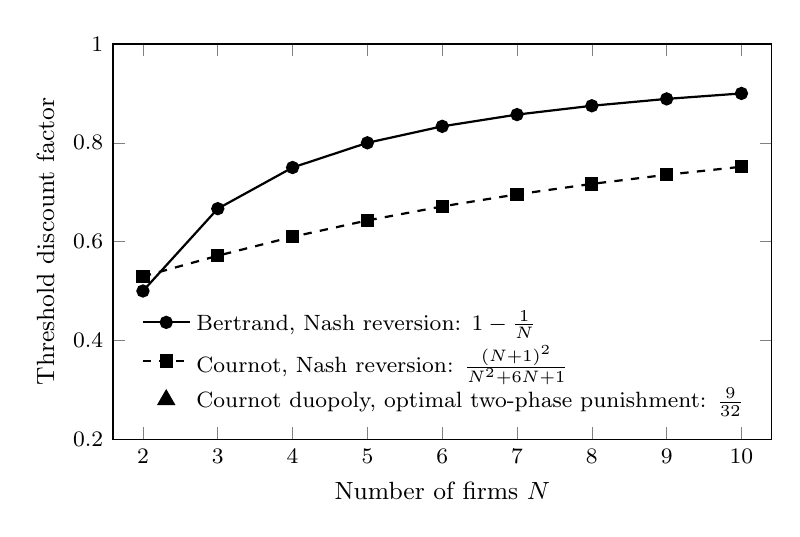
\begin{tikzpicture}
\begin{axis}[
  width=0.82\textwidth, height=6.6cm,
  xmin=1.6, xmax=10.4, ymin=0.2, ymax=1.0,
  xtick={2,3,4,5,6,7,8,9,10},
  xlabel={Number of firms $N$}, ylabel={Threshold discount factor},
  tick label style={font=\footnotesize}, label style={font=\small},
  legend style={at={(0.98,0.04)}, anchor=south east, font=\footnotesize, draw=none, fill=white},
  legend cell align=left]
\addplot[thick, mark=*, samples at={2,3,4,5,6,7,8,9,10}] {1 - 1/x};
\addlegendentry{Bertrand, Nash reversion: $1 - \frac{1}{N}$}
\addplot[thick, dashed, mark=square*, mark options={solid}, samples at={2,3,4,5,6,7,8,9,10}]
  {(x+1)^2/(x^2+6*x+1)};
\addlegendentry{Cournot, Nash reversion: $\frac{(N+1)^2}{N^2+6N+1}$}
\addplot[only marks, mark=triangle*, mark size=3.5pt] coordinates {(2,0.28125)};
\addlegendentry{Cournot duopoly, optimal two-phase punishment: $\frac{9}{32}$}
\end{axis}
\end{tikzpicture}
\caption{Minimum discount factors for collusion at the monopoly outcome. The Bertrand threshold is from
\cref{prop:12-bertrand} and the Cournot threshold, for linear demand, from \cref{prop:12-cournot}. The triangle is the
threshold for the linear Cournot duopoly with the optimal stick-and-carrot punishment of \cref{ex:12-abreu-linear}.}
\label{fig:12-critical-delta}
\end{figure}

Unlike the Bertrand supergame, the Cournot supergame allows partial collusion. When firms are too impatient to
sustain the monopoly output, they can still sustain outputs between the monopoly and Cournot levels.

\begin{proposition}[Partial collusion in linear Cournot]\label{prop:12-partial-cournot}
In the setting of \cref{prop:12-cournot}, let $\delta < \delta^*(N)$ and consider grim trigger with a symmetric
collusive output $q$ between $q^m$ and the Cournot output $q^N$. The profile is an SPE if and only if
$q \ge q(\delta)$, where
\begin{equation}\label{eq:12-partial-q}
q(\delta) = \frac{a - c}{b(N + 1)}\cdot\frac{(N + 1)^2(1 - \delta) + 4\delta}{(N + 1)^2(1 - \delta) + 4N\delta} .
\end{equation}
The output $q(\delta)$ falls continuously from $q^N$ at $\delta = 0$ to $q^m$ at $\delta = \delta^*(N)$. The most
profitable sustainable symmetric output is $q(\delta)$, and the corresponding profit rises continuously from $\pi^N$
to $\pi^c$ as $\delta$ rises from $0$ to $\delta^*(N)$.
\end{proposition}

\begin{proof}
Outputs scale with $\frac{a - c}{b}$ and profits with $k$, while the incentive constraint is homogeneous in profits.
We may therefore set $a - c = 1$ and $b = 1$ and restore the scale at the end. Then
\begin{equation*}
\pi(q) = q(1 - Nq), \qquad \pi^d(q) = \frac{\bigl[1 - (N - 1)q\bigr]^2}{4}, \qquad \pi^N = \frac{1}{(N + 1)^2} ,
\end{equation*}
where $\pi^d(q)$ follows from the best response $\frac{1 - (N - 1)q}{2}$, as in the proof of \cref{prop:12-cournot}.
The incentive constraint is $\pi^d(q) - \pi(q) \le \frac{\delta}{1 - \delta}\bigl[\pi(q) - \pi^N\bigr]$. Its left side
is
\begin{align*}
\pi^d(q) - \pi(q)
&= \frac{1 - 2(N - 1)q + (N - 1)^2q^2 - 4q + 4Nq^2}{4} \\
&= \frac{1 - 2(N + 1)q + (N + 1)^2q^2}{4}
= \frac{\bigl[1 - (N + 1)q\bigr]^2}{4} .
\end{align*}
The profit difference on the right side factors as
\begin{equation*}
\pi(q) - \pi^N = q - Nq^2 - \frac{1}{(N + 1)^2} = N\left(\frac{1}{N + 1} - q\right)\left(q - \frac{1}{N(N + 1)}\right) ,
\end{equation*}
as expanding the product confirms. Now substitute $u = 1 - (N + 1)q$, which runs from $0$ at $q = q^N$ to
$u^m = \frac{N - 1}{2N}$ at $q = q^m = \frac{1}{2N}$. Then $\frac{1}{N + 1} - q = \frac{u}{N + 1}$ and
$q - \frac{1}{N(N + 1)} = \frac{N - 1 - Nu}{N(N + 1)}$, so
\begin{equation*}
\pi(q) - \pi^N = \frac{u\,(N - 1 - Nu)}{(N + 1)^2} .
\end{equation*}
The incentive constraint becomes
\begin{equation*}
\frac{u^2}{4} \le \frac{\delta}{1 - \delta}\cdot\frac{u\,(N - 1 - Nu)}{(N + 1)^2} .
\end{equation*}
At $u = 0$ both sides vanish. For $u > 0$, multiply both sides by $\frac{4(1 - \delta)(N + 1)^2}{u} > 0$:
\begin{align*}
(1 - \delta)(N + 1)^2\,u &\le 4\delta\,(N - 1 - Nu) , \\
u\,\bigl[(1 - \delta)(N + 1)^2 + 4N\delta\bigr] &\le 4\delta(N - 1) , \\
u &\le \bar u(\delta) \equiv \frac{4\delta(N - 1)}{(1 - \delta)(N + 1)^2 + 4N\delta} .
\end{align*}
The constraint is linear in $u$, so the sustainable outputs form the interval $u \in [0, \bar u(\delta)]$, that is,
$q \ge \frac{1 - \bar u(\delta)}{N + 1}$. Since
\begin{equation*}
1 - \bar u(\delta) = \frac{(1 - \delta)(N + 1)^2 + 4N\delta - 4\delta(N - 1)}{(1 - \delta)(N + 1)^2 + 4N\delta}
= \frac{(1 - \delta)(N + 1)^2 + 4\delta}{(1 - \delta)(N + 1)^2 + 4N\delta} ,
\end{equation*}
restoring the scale gives \eqref{eq:12-partial-q}. Writing
$\bar u(\delta) = \frac{4(N - 1)}{(N + 1)^2\frac{1 - \delta}{\delta} + 4N}$ shows that $\bar u$ is continuous and
increasing, with $\bar u(0) = 0$. It reaches $u^m$ where $8N\delta = (1 - \delta)(N + 1)^2 + 4N\delta$, that is, at
$\delta = \frac{(N + 1)^2}{(N + 1)^2 + 4N} = \delta^*(N)$. Finally, $\pi(q)$ decreases in $q$ on $[q^m, q^N]$, so the
most profitable sustainable output is the smallest one, $q(\delta)$.
\end{proof}

A numerical example shows how much collusion impatient firms can sustain. Take $N = 2$ and $\delta = 0.4$, below the
threshold $\frac{9}{17}$, in units with $a - c = 1$ and $b = 1$. Then $\bar u = \frac{1.6}{5.4 + 3.2} = \frac{8}{43}$,
and the most collusive output is $q(0.4) = \frac{1 - \frac{8}{43}}{3} = \frac{35}{129} \approx 0.271$ per firm. This
lies between the monopoly-sharing output 0.25 and the Cournot output 0.333. The margin is
$P - c = 1 - \frac{70}{129} = \frac{59}{129} \approx 0.457$, and each firm earns $\frac{35}{129}\cdot\frac{59}{129}
\approx 0.1241$. Monopoly sharing would give $0.125$ and Cournot $0.1111$, so the firms sustain about 93 percent of
the gain from collusion over Cournot competition. The script \texttt{partial\_cournot.py} confirms these values by
brute force.

\begin{remark}[Repeated play and the conduct parameter]\label{rem:12-conduct}
The menu of conduct in \cref{tab:02-conduct-menu} sets $\theta = 0$ for competition, $\theta = \frac{1}{N}$ for
Cournot and $\theta = 1$ for monopoly. In the linear model the supply relation reads $P - c = \theta\,bQ$. Along the
partial-collusion frontier of \cref{prop:12-partial-cournot}, with $u = \bar u(\delta)$,
\begin{equation*}
\theta(\delta) = \frac{P - c}{bQ} = \frac{1 + N\bar u(\delta)}{N\bigl[1 - \bar u(\delta)\bigr]} ,
\end{equation*}
which rises continuously from $\frac{1}{N}$ at $\delta = 0$ to $1$ at $\delta = \delta^*(N)$. In the example above,
$\theta(0.4) = \frac{59}{70} \approx 0.84$. A conduct parameter estimated from data is thus a summary of the
equilibrium of a dynamic game. If demand or costs change over time, the most collusive equilibrium changes too, and a
constant $\theta$ averages over conduct that varies. This is the critique of \citet{Corts1999} discussed in
\cref{sec:03-corts}. With differentiated products, full collusion is joint profit maximization over all products. It
corresponds to an ownership matrix of ones, $\Omega = \mathbf{1}\mathbf{1}^\top$, in the markup equation
\eqref{eq:04-markup}. The partial internalization weights of \cref{rem:11-mc-theta} are a reduced form for
intermediate conduct.
\end{remark}

\subsection{Optimal punishments}\label{sec:12-optimal-punishment}

Nash reversion is a natural punishment, but in the Cournot game it is far from the harshest credible one. Cournot
profits are positive, while the minmax payoff is zero. \citet{Abreu1986,Abreu1988} showed how to construct the
harshest credible punishments, and that they can be described simply.

\citet{Abreu1988} proves that every SPE outcome path can be supported by a \emph{simple strategy profile}. Such a
profile consists of the desired path and one punishment path for each player. Any unilateral deviation by player
$i$, from any path, starts player $i$'s punishment path from its beginning. Simultaneous deviations by several
players are ignored. The \emph{optimal penal code} uses, for each player, a punishment path that gives that player its
lowest SPE payoff. An outcome path is then an SPE path if and only if no player gains from a one-shot deviation from
it followed by that player's lowest SPE payoff. Harsher credible punishments thus enlarge the set of sustainable
paths, and the worst punishments sustain the most.

For symmetric Cournot supergames, \citet{Abreu1986} shows that, under regularity conditions, the optimal symmetric
punishment has a two-phase \emph{stick-and-carrot} form. In the first phase all firms produce a high output $x$ for one
period, which is the stick. They then return to the most collusive symmetric path, which is the carrot.

\begin{proposition}[Two-phase punishments]\label{prop:12-abreu-two-phase}
Consider $N$ identical Cournot firms, with $\pi(q)$ and $\pi^d(q)$ defined as in \eqref{eq:12-cournot-dev}. Fix a
collusive output $q^c$ and a stick output $x$, and define a profile with two states. In state C every firm produces
$q^c$, and in state P every firm produces $x$. Play starts in state C. After any period in which some firm deviated
from the prescribed output, the next state is P. After any period without a deviation, the next state is C. The
profile is an SPE if and only if
\begin{align}
\pi^d(q^c) - \pi(q^c) &\le \delta\,\bigl[\pi(q^c) - \pi(x)\bigr] , \label{eq:12-carrot}\\
\pi^d(x) - \pi(x) &\le \delta\,\bigl[\pi(q^c) - \pi(x)\bigr] . \label{eq:12-stick}
\end{align}
\end{proposition}

\begin{proof}
We use unnormalized values. The value of state C is $V_C = \frac{\pi(q^c)}{1 - \delta}$, since without deviations the
game stays in C. The value of state P is one period of the stick followed by the carrot, $V_P = \pi(x) + \delta V_C$.
By \cref{prop:12-osdp} we only need to rule out one-shot deviations in each state, and every deviation leads to P.

In state C, the best one-shot deviation earns $\pi^d(q^c)$ and moves the game to P. It is unprofitable if and only if
$\pi^d(q^c) + \delta V_P \le V_C$. Using the expressions for $V_C$ and $V_P$,
\begin{equation*}
V_C - \delta V_P = \frac{\pi(q^c)}{1 - \delta} - \delta\pi(x) - \frac{\delta^2\pi(q^c)}{1 - \delta}
= (1 + \delta)\,\pi(q^c) - \delta\,\pi(x) .
\end{equation*}
The condition $\pi^d(q^c) \le (1 + \delta)\pi(q^c) - \delta\pi(x)$ is \eqref{eq:12-carrot}.

In state P, the best one-shot deviation earns $\pi^d(x)$ and restarts the stick, so the game is again in P. It is
unprofitable if and only if $\pi^d(x) + \delta V_P \le V_P$, that is,
\begin{equation*}
\pi^d(x) \le (1 - \delta)V_P = (1 - \delta)\,\pi(x) + \delta\,\pi(q^c) .
\end{equation*}
Subtracting $\pi(x)$ from both sides gives \eqref{eq:12-stick}.
\end{proof}

The two constraints have clear meanings. The \emph{carrot constraint} \eqref{eq:12-carrot} says that the one-period
gain from cheating on the collusive output must not exceed the loss from spending one period in the stick instead of
the carrot. The \emph{stick constraint} \eqref{eq:12-stick} says that firms must be willing to carry out the
punishment. During the stick each firm would like to cut its output and enjoy the higher price. It refrains because a
deviation would restart the stick and delay the return to collusion. The normalized value of the punishment is
$(1 - \delta)\pi(x) + \delta\pi(q^c)$. The stick can impose a stage profit below the minmax payoff, even a loss. By
\eqref{eq:12-stick}, however, the value of the whole punishment is at least $\pi^d(x)$, which is at least the minmax
payoff.

\begin{example}[Stick and carrot in the linear Cournot duopoly]\label{ex:12-abreu-linear}
Two firms with constant marginal cost $c \ge 0$ face the inverse demand $P(Q) = a - Q$ for every $Q \ge 0$, with
$a > c$. Outputs scale with $a - c$ and profits with $(a - c)^2$, and the thresholds on $\delta$ do not depend on the
scale, so we set $a - c = 1$. The collusive output is $q^c = q^m = \frac{1}{4}$, with
\begin{equation*}
\pi(q^m) = \frac{1}{4}\cdot\frac{1}{2} = \frac{1}{8}, \qquad
\pi^d(q^m) = \left(\frac{1 - \frac{1}{4}}{2}\right)^2 = \frac{9}{64}, \qquad
\pi^d(q^m) - \pi(q^m) = \frac{1}{64} .
\end{equation*}
For a stick output $x \le 1$, the stage profit is $\pi(x) = x(1 - 2x)$ and the best response to $x$ is
$\frac{1 - x}{2}$, so $\pi^d(x) = \frac{(1 - x)^2}{4}$. The gain from deviating during the stick and the loss from the
stick are
\begin{align*}
\pi^d(x) - \pi(x) &= \frac{1 - 2x + x^2 - 4x + 8x^2}{4} = \frac{(3x - 1)^2}{4} , \\
\pi(q^m) - \pi(x) &= \frac{1 - 8x + 16x^2}{8} = \frac{(4x - 1)^2}{8} .
\end{align*}
For $x \ne \frac{1}{4}$, constraints \eqref{eq:12-carrot} and \eqref{eq:12-stick} become $\delta \ge \delta_C(x)$ and
$\delta \ge \delta_S(x)$, with
\begin{equation*}
\delta_C(x) = \frac{\frac{1}{64}}{\frac{(4x - 1)^2}{8}} = \frac{1}{8(4x - 1)^2} , \qquad
\delta_S(x) = \frac{\frac{(3x - 1)^2}{4}}{\frac{(4x - 1)^2}{8}} = \frac{2(3x - 1)^2}{(4x - 1)^2} .
\end{equation*}
For $x < \frac{1}{4}$ the stick raises the price. Then
$\delta_S(x) = 2\left(\frac{1 - 3x}{1 - 4x}\right)^2 \ge 2$, because $1 - 3x \ge 1 - 4x > 0$, so no such stick
works. We therefore take $x > \frac{1}{4}$. A harsher stick lowers $\delta_C$. Beyond the Cournot output $x = \frac{1}{3}$, it raises $\delta_S$, because the
ratio $\frac{3x - 1}{4x - 1}$ has derivative $\frac{1}{(4x - 1)^2} > 0$. On $(\frac{1}{4}, \frac{1}{3}]$ no stick
works, since $\delta_C(x) \ge \delta_C(\frac{1}{3}) = \frac{9}{8} > 1$. For $x \ge 1$ the best response is zero, and
$\delta_S(x) = \frac{2x^2 - x}{2x^2 - x + \frac{1}{8}} \ge \frac{8}{9}$. The lowest discount factor that some stick
can support is therefore attained where the two curves cross on $(\frac{1}{3}, 1)$:
\begin{align*}
\frac{(3x - 1)^2}{4} &= \frac{1}{64} , \\
(3x - 1)^2 &= \frac{1}{16} , \\
48x^2 - 32x + 5 &= 0 .
\end{align*}
The roots are $x = \frac{1}{4}$, which is the collusive output itself, and $x = \frac{5}{12}$. At $x = \frac{5}{12}$,
\begin{equation*}
\pi(x) = \frac{5}{12}\cdot\frac{1}{6} = \frac{5}{72}, \qquad
\pi(q^m) - \pi(x) = \frac{9}{72} - \frac{5}{72} = \frac{1}{18}, \qquad
\underline\delta = \frac{\frac{1}{64}}{\frac{1}{18}} = \frac{18}{64} = \frac{9}{32} .
\end{equation*}
In general units the stick output is $x = \frac{5(a - c)}{12}$ per firm. The stick price is
$\frac{a + 5c}{6}$, still above marginal cost, and each firm earns $\frac{5(a - c)^2}{72}$, below the Cournot profit
$\frac{8(a - c)^2}{72}$. The optimal two-phase punishment sustains monopoly for $\delta \ge \frac{9}{32} \approx
0.281$, against $\frac{9}{17} \approx 0.529$ with Nash reversion. A grid search in \texttt{abreu\_check.py} over
stick outputs confirms the threshold and the stick output for several values of $c$.
\end{example}

\begin{figure}[htbp]
\centering
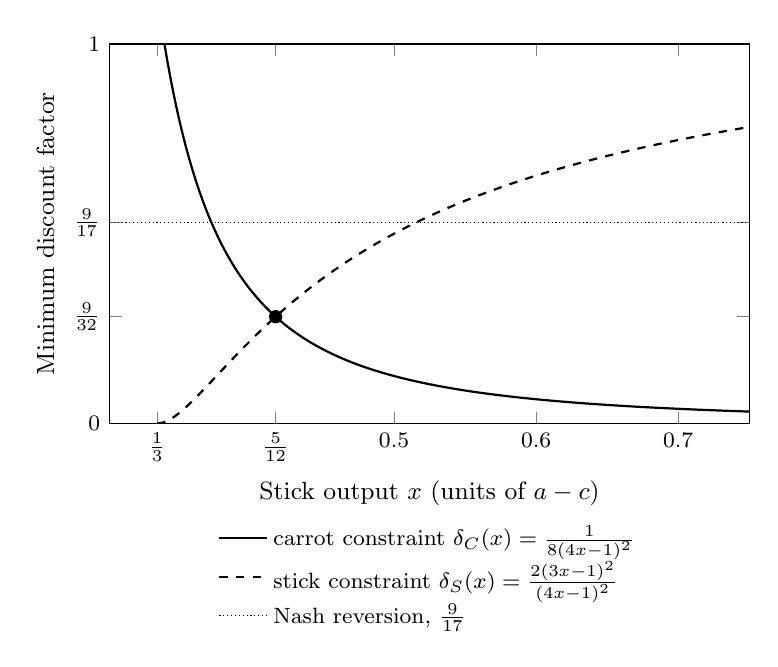
\begin{tikzpicture}
\begin{axis}[
  width=0.8\textwidth, height=6.4cm,
  xmin=0.30, xmax=0.75, ymin=0, ymax=1.0,
  xtick={0.33333,0.41667,0.5,0.6,0.7},
  xticklabels={$\frac{1}{3}$,$\frac{5}{12}$,$0.5$,$0.6$,$0.7$},
  ytick={0,0.28125,0.5294,1},
  yticklabels={$0$,$\frac{9}{32}$,$\frac{9}{17}$,$1$},
  xlabel={Stick output $x$ (units of $a - c$)}, ylabel={Minimum discount factor},
  tick label style={font=\footnotesize}, label style={font=\small},
  legend style={at={(0.5,-0.24)}, anchor=north, font=\footnotesize, draw=none, fill=white},
  legend cell align=left]
\addplot[thick, domain=0.3384:0.75, samples=200] {1/(8*(4*x-1)^2)};
\addlegendentry{carrot constraint $\delta_C(x) = \frac{1}{8(4x - 1)^2}$}
\addplot[thick, dashed, domain=0.33334:0.75, samples=200] {2*(3*x-1)^2/(4*x-1)^2};
\addlegendentry{stick constraint $\delta_S(x) = \frac{2(3x - 1)^2}{(4x - 1)^2}$}
\addplot[densely dotted, domain=0.30:0.75] {9/17};
\addlegendentry{Nash reversion, $\frac{9}{17}$}
\addplot[only marks, mark=*, mark size=2.2pt] coordinates {(0.41667,0.28125)};
\end{axis}
\end{tikzpicture}
\caption{The two constraints of the stick-and-carrot punishment in the linear Cournot duopoly with inverse demand
$a - Q$, from \cref{ex:12-abreu-linear}. A stick output $x$ supports monopoly sharing for every $\delta$ above both
curves. The best stick, $x = \frac{5(a - c)}{12}$, equates the two constraints at $\delta = \frac{9}{32}$.}
\label{fig:12-abreu}
\end{figure}

\Cref{fig:12-abreu} draws the two constraints. A harsher stick makes cheating on the cartel less attractive, but it
also makes the punishment harder to enforce. The best stick balances the two.

\begin{remark}[The price floor and the limit of punishment]\label{rem:12-abreu-floor}
\Cref{ex:12-abreu-linear} treats inverse demand as linear for all outputs, so that very large outputs would drive the
price below zero. The optimal stick keeps the price above marginal cost, but the assumption still matters, because it
determines which sticks are available. Suppose instead that the price cannot fall below zero,
$P(Q) = \max\{a - Q, 0\}$. With $c = 0$, each firm producing at least $a$ drives the price to zero at no cost.
Deviating during such a stick cannot raise the price, so the stick constraint is slack. The carrot constraint
becomes $\frac{1}{64} \le \frac{\delta}{8}$, that is, $\delta \ge \frac{1}{8}$. With $c > 0$, a stick that floods the
market costs $cx$ per period. Our computations with \texttt{abreu\_check.py} show that flooding sticks beat
$\frac{9}{32}$ only when $c < 0.051(a - c)$. Suppose $0 < c \le \frac{a - c}{64}$. A flooding stick in which each
firm produces $\frac{(a - c)^2}{64c}$, earning $-\frac{(a - c)^2}{64}$ per period, then reaches $\delta = \frac{1}{9}$,
provided outputs this large are feasible. At $c = 0$ a stick cannot impose a loss, and the best two-phase code
reaches only $\frac{1}{8}$. No equilibrium can do better than $\frac{1}{9}$. By \cref{lem:12-ir} a deviator's continuation value is at least
the minmax payoff zero, so sustaining monopoly sharing requires $\frac{\pi(q^m)}{1 - \delta} \ge \pi^d(q^m)$, that is,
$\delta \ge 1 - \frac{8}{9} = \frac{1}{9}$. The general lesson is that the harshness of credible punishments depends on
how much damage firms can inflict on one another in a period, and at what cost to themselves.
\end{remark}

In the Bertrand supergame optimal punishments add nothing. Bertrand reversion already holds every firm to its minmax
payoff of zero, which no equilibrium can undercut. Two broader lessons follow from Abreu's analysis. First, the
sustainability of collusion depends on the severity of credible punishments as well as on patience. Second, the most
effective punishment is a short, sharp price war followed by a return to collusion. Wars of this kind reappear in the
models of imperfect monitoring (\cref{sec:12-public}) and in the model of imperfect cartels of \citet{BernheimMadsen2017}
(\cref{sec:13-imperfect}). Stick-and-carrot schemes have one weakness. Once a deviation has occurred, all firms would
gain by skipping the stick and returning to collusion at once. Punishments that are immune to such renegotiation are
milder, which limits how much collusion they can sustain \citep{FarrellMaskin1989}.

\subsection{Asymmetric firms}\label{sec:12-asymmetries}

Symmetric models hide a problem that real cartels face: firms differ, and the collusive agreement must satisfy every
firm's incentive constraint. Consider two Bertrand firms with marginal costs $c_1 < c_2$, and write
$\pi_i(p) = (p - c_i)D(p)$ and $p^m(c_i)$ for firm $i$'s monopoly price. Suppose $c_2 < p^m(c_1)$, so that the cost
advantage is not drastic. The static Bertrand equilibrium then has firm 1 serving the market at a price equal to
$c_2$. Firm 1 earns $\pi_1(c_2) = (c_2 - c_1)D(c_2) > 0$ and firm 2 earns nothing. Let the firms collude on a common
price $p \in (c_2, p^m(c_1)]$ and divide the customers in shares $\alpha_1$ and $\alpha_2 = 1 - \alpha_1$. Undercutting
gives either firm the whole market for one period. With Nash reversion, the normalized incentive constraints are
\begin{equation}\label{eq:12-asym-cost}
\alpha_1\,\pi_1(p) \ge (1 - \delta)\,\pi_1(p) + \delta\,\pi_1(c_2) ,
\qquad
\alpha_2\,\pi_2(p) \ge (1 - \delta)\,\pi_2(p) .
\end{equation}
The efficient firm fears punishment less than its rival, because it keeps a positive profit in the price war. Its
constraint requires $\alpha_1 \ge 1 - \delta + \delta\psi_1$, where $\psi_1 = \frac{\pi_1(c_2)}{\pi_1(p)} \in (0, 1)$,
while firm 2 needs $\alpha_2 \ge 1 - \delta$. Adding the two requirements and using $\alpha_1 + \alpha_2 = 1$ gives
\begin{equation*}
1 \ge 2(1 - \delta) + \delta\psi_1
\quad\Longleftrightarrow\quad
\delta \ge \frac{1}{2 - \psi_1} .
\end{equation*}
The threshold exceeds the symmetric value $\frac{1}{2}$ and rises with the cost gap, which raises $\psi_1$. The cartel
must also give the efficient firm a larger share of the market. In addition, the firms disagree about the price,
since the low-cost firm prefers a lower monopoly price than the high-cost firm.

Without side payments, the firms can still trade price against market share. \citet[section~6.3.2.4,
Exercises~6.1 and~6.5]{Tirole1988} characterizes the efficient trade. Fix a profit target $\bar\pi_2 > 0$ for firm 2.
Both firms charge the price $p$, and firm $i$ produces $s_iD(p)$, with $s_1 + s_2 = 1$. A \emph{constrained-efficient
market-sharing allocation} maximizes firm 1's profit given firm 2's target:
\begin{equation}\label{eq:12-asym-frontier}
\max_{p,\, s_1,\, s_2}\; (p - c_1)\,s_1D(p)
\quad\text{subject to}\quad (p - c_2)\,s_2D(p) \ge \bar\pi_2 , \qquad s_1 + s_2 = 1 .
\end{equation}
Varying $\bar\pi_2$ traces the frontier of profit pairs that the firms can reach without transfers.

\begin{proposition}[Market sharing without side payments]\label{prop:12-asym-sharing}
Let $D$ be positive and decreasing, and let $(p - c)D(p)$ be strictly concave in $p$ for every $c$. Suppose that the
solution of \eqref{eq:12-asym-frontier} has $p > c_2$. Then:
\begin{enumerate}[label=(\roman*)]
\item The price lies between the two monopoly prices, $p^m(c_1) \le p \le p^m(c_2)$.
\item The price solves
\begin{equation}\label{eq:12-asym-foc}
\bigl[(p - c_1)D'(p) + D(p)\bigr] + \frac{(c_2 - c_1)\,\bar\pi_2}{(p - c_2)^2} = 0 .
\end{equation}
\item The price $p$ and firm 2's share $s_2$ both rise with the target $\bar\pi_2$.
\end{enumerate}
\end{proposition}

\begin{proof}
The constraint binds at the optimum, because otherwise moving share to firm 1 raises firm 1's profit. Hence
$s_2 = \frac{\bar\pi_2}{(p - c_2)D(p)}$, and firm 1's profit as a function of $p$ alone is
\begin{equation*}
\Pi_1(p) = (p - c_1)D(p)\,\Bigl[1 - \frac{\bar\pi_2}{(p - c_2)D(p)}\Bigr]
= (p - c_1)D(p) - \frac{(p - c_1)\,\bar\pi_2}{p - c_2} .
\end{equation*}
(i) Strict concavity implies $p^m(c_1) < p^m(c_2)$. For $p < p^m(c_1)$, both $(p - c_1)D(p)$ and $(p - c_2)D(p)$ rise
with $p$. Both factors in the first expression for $\Pi_1$ are then positive and rising, so $\Pi_1$ rises. For
$p > p^m(c_2)$, both factors fall, so $\Pi_1$ falls. The optimum therefore lies in $[p^m(c_1), p^m(c_2)]$.

(ii) The derivative of the last term uses
\begin{equation*}
\frac{\dd}{\dd p}\,\frac{p - c_1}{p - c_2} = \frac{(p - c_2) - (p - c_1)}{(p - c_2)^2} = -\frac{c_2 - c_1}{(p - c_2)^2} .
\end{equation*}
Setting $\Pi_1'(p) = 0$ gives \eqref{eq:12-asym-foc}.

(iii) Let $\Phi(p, \bar\pi_2)$ be the left side of \eqref{eq:12-asym-foc}. The bracket falls with $p$ by strict
concavity, and the second term falls with $p$ for $p > c_2$, so $\frac{\partial\Phi}{\partial p} < 0$. Also
$\frac{\partial\Phi}{\partial\bar\pi_2} = \frac{c_2 - c_1}{(p - c_2)^2} > 0$. By the implicit function theorem,
\begin{equation*}
\frac{\dd p}{\dd\bar\pi_2} = -\frac{\partial\Phi}{\partial\bar\pi_2}\left(\frac{\partial\Phi}{\partial p}\right)^{-1} > 0 .
\end{equation*}
For the share, solve \eqref{eq:12-asym-foc} for $\bar\pi_2$ and substitute it into $s_2$:
\begin{equation*}
s_2 = \frac{-\bigl[(p - c_1)D'(p) + D(p)\bigr]\,(p - c_2)}{(c_2 - c_1)\,D(p)} .
\end{equation*}
On $[p^m(c_1), p^m(c_2)]$ the factor $-[(p - c_1)D'(p) + D(p)]$ is nonnegative and rising, $p - c_2$ is positive and
rising, and $\frac{1}{D(p)}$ is positive and rising. Their product rises with $p$, and hence with $\bar\pi_2$.
\end{proof}

The proposition shows how a cartel without transfers compensates the high-cost firm. To give firm 2 more profit, it
raises the price toward firm 2's preferred level and also gives firm 2 more of the market. Both moves sacrifice
industry profit, because the efficient allocation would let firm 1 serve the market at $p^m(c_1)$. The comparison with
\eqref{eq:12-asym-cost}, where the price was fixed at or below $p^m(c_1)$, shows that efficient sharing uses higher
prices.

Which points of this frontier can grim trigger sustain? Let $\pi_i^*$ be firm $i$'s collusive profit at an
allocation. Firm 1's best deviation charges its own monopoly price $p^m(c_1) \le p$, takes the whole market and earns
$\pi_1(p^m(c_1))$. Bertrand reversion then leaves it $\pi_1(c_2)$ per period. Firm 2's best deviation undercuts $p$
slightly and earns almost $(p - c_2)D(p)$, and reversion leaves it zero. The two constraints are
\begin{equation}\label{eq:12-asym-ic}
\pi_1\bigl(p^m(c_1)\bigr) - \pi_1^* \;\le\; \frac{\delta}{1 - \delta}\bigl[\pi_1^* - \pi_1(c_2)\bigr],
\qquad
(p - c_2)D(p) - \pi_2^* \;\le\; \frac{\delta}{1 - \delta}\,\pi_2^* .
\end{equation}
The first holds only if firm 1's collusive profit is high enough, and the second only if firm 2's is. For a given
$\delta$ only a middle segment of the frontier is sustainable. This is the counterpart, with a variable price, of
\eqref{eq:12-asym-cost}. Tirole adds that the choice among these allocations is itself a coordination problem, which
no symmetry argument can settle when costs differ (section~6.3.2.4).

Capacity asymmetries work through both sides of the constraint. A firm with spare capacity gains much from undercutting
and is hard to punish, because its small rivals cannot flood the market (\cref{ex:12-capacity} and
\citealp{CompteJennyRey2002}). A firm whose incentive constraint is the hardest to satisfy, because of low costs, spare
capacity, or a small share of the collusive profits, constrains what the whole group can sustain. Merger guidelines
call a firm that plays this disruptive role a \emph{maverick} \citep{USDOJFTC2010}. Product differentiation is a
further source of asymmetry, and the next subsection studies its symmetric version.

\subsection{Differentiated products}\label{sec:12-diffprod}

With differentiated products, a firm that undercuts its rivals gains some of their customers but not all, and the
static Nash equilibrium yields positive profits. Both the temptation and the punishment become milder. We work out a
linear duopoly in which the two effects can be compared in closed form.

\begin{proposition}[Collusion with differentiated products]\label{prop:12-diffprod}
Two firms with zero marginal cost face demands $q_i = 1 - p_i + s\,p_j$ for $i \ne j$, with
$0 \le s \le \sqrt 3 - 1 \approx 0.73$. Here $s$ measures substitutability and is not a market share. With grim
trigger and Bertrand-Nash reversion, the joint-profit price is sustainable if and only if
\begin{equation}\label{eq:12-diffprod-delta}
\delta \ge \underline\delta(s) \equiv \frac{(2 - s)^2}{s^2 - 8s + 8} .
\end{equation}
The threshold increases in $s$, from $\frac{1}{2}$ at $s = 0$ to $\frac{3}{5}$ at $s = \sqrt 3 - 1$.
\end{proposition}

\begin{proof}
The model is \cref{ex:04-linear-duopoly} with $a = b = 1$, $d = s$ and $c = 0$. We compute the three profits.

We start with the static Nash equilibrium. Firm $i$ maximizes $p_i(1 - p_i + sp_j)$. The first-order condition
$1 - 2p_i + sp_j = 0$ gives the symmetric equilibrium price $p^N = \frac{1}{2 - s}$. Each firm sells
$1 - (1 - s)p^N = \frac{1}{2 - s}$, so $\pi^N = \frac{1}{(2 - s)^2}$.

Under collusion the firms choose a common price $p$ to maximize $2p\bigl[1 - (1 - s)p\bigr]$. The first-order
condition $1 - 2(1 - s)p = 0$ gives $p^c = \frac{1}{2(1 - s)}$. Each firm sells $\frac{1}{2}$, so
$\pi^c = \frac{1}{4(1 - s)}$.

A firm $i$ that deviates against $p^c$ maximizes $p_i(1 - p_i + sp^c)$, so
\begin{equation*}
p^d = \frac{1 + sp^c}{2} = \frac{1}{2}\left[1 + \frac{s}{2(1 - s)}\right] = \frac{2 - s}{4(1 - s)} .
\end{equation*}
Its sales equal its price, $1 - p^d + sp^c = p^d$, so $\pi^d = (p^d)^2 = \frac{(2 - s)^2}{16(1 - s)^2}$. At this
price the rival sells
\begin{equation*}
1 - p^c + s\,p^d = \frac{4(1 - s) - 2 + s(2 - s)}{4(1 - s)} = \frac{2 - 2s - s^2}{4(1 - s)} ,
\end{equation*}
which is nonnegative if and only if $s \le \sqrt 3 - 1$. For larger $s$ the linear system would assign the rival
negative sales, and the deviation must be computed with the rival's demand truncated at zero.

The threshold \eqref{eq:12-cournot-ic} applies with these profits. The two differences are
\begin{align*}
\pi^d - \pi^c &= \frac{(2 - s)^2 - 4(1 - s)}{16(1 - s)^2} = \frac{s^2}{16(1 - s)^2} , \\
\pi^d - \pi^N &= \frac{(2 - s)^4 - 16(1 - s)^2}{16(1 - s)^2(2 - s)^2}
= \frac{s^2\,(s^2 - 8s + 8)}{16(1 - s)^2(2 - s)^2} ,
\end{align*}
where the second line uses the factorization
\begin{equation*}
(2 - s)^4 - 16(1 - s)^2 = \bigl[(2 - s)^2 - 4(1 - s)\bigr]\bigl[(2 - s)^2 + 4(1 - s)\bigr] = s^2\,(s^2 - 8s + 8) .
\end{equation*}
Their ratio is \eqref{eq:12-diffprod-delta}. The quadratic $s^2 - 8s + 8$ has roots $4 \pm 2\sqrt 2$, both outside $[0, 1]$, so it is
positive on $[0, 1]$. Differentiating,
\begin{equation*}
\frac{d\underline\delta}{ds}
= \frac{-2(2 - s)(s^2 - 8s + 8) - (2 - s)^2(2s - 8)}{(s^2 - 8s + 8)^2}
= \frac{4s(2 - s)}{(s^2 - 8s + 8)^2} > 0
\end{equation*}
for $s \in (0, 1)$. At $s = 0$ the threshold is $\frac{4}{8} = \frac{1}{2}$. At $s = \sqrt 3 - 1$ we have
$(2 - s)^2 = 12 - 6\sqrt 3$ and $s^2 - 8s + 8 = 20 - 10\sqrt 3$, so the threshold is
$\frac{6(2 - \sqrt 3)}{10(2 - \sqrt 3)} = \frac{3}{5}$.
\end{proof}

\begin{figure}[htbp]
\centering
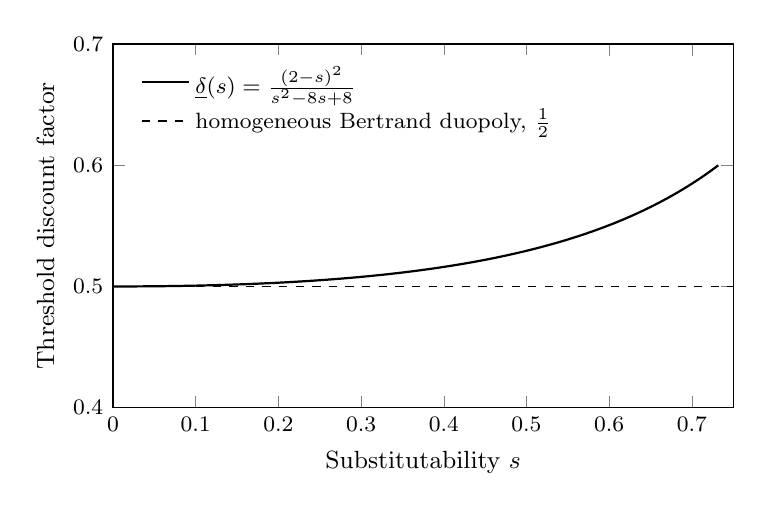
\begin{tikzpicture}
\begin{axis}[
  width=0.78\textwidth, height=6.2cm,
  xmin=0, xmax=0.75, ymin=0.4, ymax=0.7,
  xlabel={Substitutability $s$}, ylabel={Threshold discount factor},
  tick label style={font=\footnotesize}, label style={font=\small},
  legend style={at={(0.03,0.97)}, anchor=north west, font=\footnotesize, draw=none, fill=white},
  legend cell align=left]
\addplot[thick, domain=0:0.732, samples=150] {(2-x)^2/(x^2-8*x+8)};
\addlegendentry{$\underline\delta(s) = \frac{(2 - s)^2}{s^2 - 8s + 8}$}
\addplot[dashed, domain=0:0.75] {0.5};
\addlegendentry{homogeneous Bertrand duopoly, $\frac{1}{2}$}
\end{axis}
\end{tikzpicture}
\caption{Minimum discount factor for collusion at the joint-profit price in the linear differentiated duopoly
$q_i = 1 - p_i + s\,p_j$ with zero cost and Bertrand-Nash reversion (\cref{prop:12-diffprod}).}
\label{fig:12-diffprod-delta}
\end{figure}

\Cref{fig:12-diffprod-delta} plots the threshold. In this specification collusion is easier when products are more
differentiated. Both the gain from deviating and the loss from punishment vanish as $s \to 0$, since
\begin{equation*}
\pi^d - \pi^c = \frac{s^2}{16(1 - s)^2}, \qquad \pi^c - \pi^N = \frac{s^2}{4(1 - s)(2 - s)^2} .
\end{equation*}
The threshold depends on their ratio $R(s) = \frac{(2 - s)^2}{4(1 - s)}$, because
$\underline\delta = \frac{\pi^d - \pi^c}{(\pi^d - \pi^c) + (\pi^c - \pi^N)} = \frac{R}{1 + R}$. The ratio equals one at
$s = 0$ and rises with $s$, so closer substitutes raise the temptation faster than they raise the punishment.
\citet[eq.~(21)]{Deneckere1983} and \citet[eq.~(8)]{Ross1992} derive the same threshold. They state it as the highest
interest rate at which collusion survives, $\frac{1 - \underline\delta}{\underline\delta} = \frac{1}{R(s)} =
\frac{4(1 - s)}{(2 - s)^2}$. Deneckere measures substitutability by the cross-to-own ratio in inverse demand, which
equals $-s$ in our model. Substituting $-s$ for his parameter turns his eq.~(21) into this expression.

Two cautions apply. First, the closed form holds only for $s \le \sqrt 3 - 1$. Beyond that point the deviator's best
price would drive the rival's linear demand below zero. The deviator can take at most the rival's whole market, so
its best deviation then leaves the rival with exactly zero sales. \citet[pp.~40--42]{Deneckere1983} and
\citet[p.~7]{Ross1992} show that with this cap the threshold stops rising. \citet[p.~7]{Ross1992} puts the turning
point near $s = 0.77$. His eq.~(9) gives a highest interest rate of $0.64$ there, so the threshold is
$\frac{1}{1.64} \approx 0.61$. The threshold then falls back toward the homogeneous Bertrand value $\frac{1}{2}$
as $s \to 1$, so the relation is non-monotone over the full range. Second, the answer depends on the model of differentiation. Within the linear
model the threshold depends only on the ratio of the cross-price to the own-price effect, which is $s$ here. The
scale of demand does not matter \citep[p.~7]{Ross1992}. In a spatial model with linear transport costs, where the best
deviation steals only marginal customers, the threshold falls as transport costs rise. A cartel of differentiated
products can then be more stable than one of identical products \citep[pp.~8--11]{Ross1992}.
The general point survives. Differentiation weakens both the temptation to cheat and the punishment, and which effect
dominates depends on the specific model of differentiation \citep[p.~5]{Ross1992}.

\subsection{Coordinated effects of mergers}\label{sec:12-coordinated}

The theory of this section supplies the economics behind the \emph{coordinated effects} of mergers
(\cref{def:11-coordinated}). A merger can make collusion easier through three channels. It removes a firm, which
lowers the threshold. In the Bertrand supergame a merger from $N$ to $N - 1$ firms lowers it from $1 - \frac{1}{N}$
to $1 - \frac{1}{N - 1}$, for example from 0.75 to 0.67 when four firms become three. In the linear Cournot
supergame a merger from three firms to two lowers $\delta^*$ from $\frac{4}{7} \approx 0.571$ to
$\frac{9}{17} \approx 0.529$. In the Bertrand supergame the deviation profit, which is the monopoly profit, and the
punishment profit, which is zero, do not depend on the number of firms. In richer models both fall as firms are
added. A merger then raises both sides of the incentive constraint, and its effect on the threshold is ambiguous in
general \citep[p.~239]{AskerNocke2021}. In the linear Cournot case the net effect lowers the threshold, as the
numbers above show. A merger also changes
asymmetries, and the model of \citet{CompteJennyRey2002} shows how. When the firms other than the largest can serve
the market, the threshold \eqref{eq:12-cjr} is $\frac{\hat K - 1}{\hat K}$, and a merger can only lower it. When
they cannot, the threshold \eqref{eq:12-cjr-large} is $\frac{\hat k_N}{\hat K}$. A merger involving the largest firm
then raises it, while a merger among smaller firms that leaves the largest firm unchanged has no effect. A merger that
creates a large firm with spare capacity, or that gives the merged firm a cost advantage, can thus create a maverick
and make collusion harder. Finally, a merger can eliminate a maverick, which is the case that merger guidelines
emphasize \citep{USDOJFTC2010}. Because the theory has many equilibria, it identifies the conditions under which
coordination is feasible after a merger. It cannot tell us whether coordination will occur. \Cref{sec:11-millercoors}
studies the evidence from the MillerCoors joint venture, where post-merger prices are consistent with coordination
\citep{MillerWeinberg2017}.

Entry interacts with collusion as well. Under perfect collusion with free entry, firms enter until the collusive
profit per firm equals the fixed cost. In the linear Cournot model with a fixed cost $\Phi$ per firm and period,
collusion supports $N^m = \frac{(a - c)^2}{4b\Phi}$ firms, at least as many as Cournot competition with free entry.
Entry then dissipates the whole monopoly rent (\cref{sec:C-cournot}). Consumers gain nothing, because the price stays at the monopoly level. The larger number
of firms also raises the discount factor that collusion requires, since $\delta^*(N^m) > \delta^*(N)$ for any smaller
$N$. Under full collusion the Lerner index is $\frac{a - c}{a + c}$ whatever the number of firms,
so concentration and margins are unrelated under collusion. Cross-industry regressions of margins on concentration
therefore mix industries whose margins respond to concentration (Cournot) with industries whose margins do not
(collusion), as \cref{sec:02-LH,sec:C-cournot} show.
